\documentclass[12pt]{extreport}

\usepackage{lipsum}

\usepackage[utf8]{vietnam}
\usepackage{graphicx}

\usepackage{mathptmx}

\usepackage{indentfirst}

\usepackage[
    a4paper,
    left=3cm, % lề trái
    right=2cm, % lề phải
    bottom=3cm, % lề dưới
    top=2.5cm % lề trên
]{geometry}

\usepackage{setspace}
\setstretch{1.3}

\graphicspath{ {images/} }

\title{Title}
\author{Author Name}
\date{Day Month Year}

\begin{document}

\maketitle

\pagenumbering{roman}

\addcontentsline{toc}{chapter}{PHÊ DUYỆT CỦA GIẢNG VIÊN HƯỚNG DẪN}
\chapter*{Phê duyệt của giảng viên hướng dẫn}
\addcontentsline{toc}{chapter}{PHÊ DUYỆT CỦA GIẢNG VIÊN HƯỚNG DẪN}
\chapter*{Phê duyệt của giảng viên hướng dẫn}

Tôi xác nhận rằng dự án đến hiện tại đã sẵn sàng cho hội đồng thẩm định để lấy bằng cử nhân ngành Khoa học Máy tính trường Đại học Công nghệ.

\begin{flushright}
Ký tên:..................................................................................

Th.S Hồ Đắc Phương

Cán bộ hướng dẫn dự án

Khoa Công nghệ thông tin

Trường Đại học Công Nghệ

Đại học Quốc gia Hà Nội
\end{flushright}


\addcontentsline{toc}{chapter}{LỜI MỞ ĐẦU}
\chapter*{Lời mở đầu}
Trước tiên, tôi xin bày tỏ lòng biết ơn chân thành và sâu sắc nhất đến thầy giáo, Th.S Hồ Đắc Phương, người đã tận tình chỉ bảo, hướng dẫn, động viên và giúp đỡ tôi trong suốt quá trình làm học phần dự án. Kiến thức và kinh nghiệm nghiên cứu tôi có được từ thầy sẽ rất quan trọng đối với tương lai của tôi.

Tiếp theo, em xin gửi đến quý thầy cô giáo trong ngành Khoa học máy tính, Khoa Công nghệ Thông tin nói riêng và trong Trường Đại học Công nghệ - Đại học Quốc Gia Hà Nội nói chung đã dành tâm huyết của mình để truyền đạt vốn kiến thức quý báu cho chúng em trong suốt thời gian học tập tại trường. Các thầy cô không chỉ giảng dạy mà còn định hướng cho em rất hiều trong quá trình phát triển bản thân và trong cuộc sống. Bên cạnh đó tôi cũng gửi lời cảm ơn đến anh, chị, em, bạn bè đã đồng hành cùng tôi suốt những năm dưới mái trường đại học Công Nghệ.

Tiếp đến, tôi xin được cảm ơn gia đình, đã sinh thành và nuôi dưỡng cũng như định hướng, động viên tôi trong suốt quá trình học tập.

Cuối cùng, báo cáo dự án này không tránh khỏi những thiếu sót. Tôi mong nhận được những nhận xét về những sai sót và ý kiến đóng góp để dự án hoàn thiện hơn.

Tôi xin chân thành cảm ơn!

\begin{flushright}
Hà Nội, ngày tháng năm 2021

\textbf{Sinh viên}

\bigskip
\bigskip

\textbf{Lê Tiến Chiến}
\end{flushright}


\addcontentsline{toc}{chapter}{TÓM TẮT}
\chapter*{Tóm tắt}
\addcontentsline{toc}{chapter}{TÓM TẮT}
\chapter*{Tóm tắt}

Ngày này có rất nhiều hệ thống được xây dựng dựa trên các mô hình tính toán khác nhau.
Với mỗi mô hình tính toán lại có các ưu, nhược điểm khác nhau.
Để đánh giá mỗi mô hình tính toán, cần triển khai mỗi mô hình trên hệ thống trong một thời gian dài.
Sau khi triển khai xong, các doanh nghiệp tổ chức rất khó để so sánh giữa các mô hình tính toán khác nhau.
Bởi vì mỗi mô hình được chạy trong các khoảng thời gian khác nhau và có tập người sử dụng khác nhau
trong các thời điểm.

Do đó các doanh nghiệp nảy sinh ra nhu cầu cần có một hệ thống toàn diện để giải quyết bài toán trên.
Hệ thống này có thể đánh giá các mô hình tính toán khác nhau một cách chính xác và công bằng.
Từ đó doanh nghiệp có thể biết được mô hình tính toán nào tốt hơn mà không cần phải tốn quá nhiều
thời gian thử nghiệm trên từng mô hình.

Hệ thống A/B Testing được ra đời để hoàn thành mục đích đó. Khi sử dụng hệ thống, bất cứ người dùng
nào cũng có thể khởi tạo các mô hình với các thông số khác nhau để so sánh. Hệ thống A/B Testing cũng
có thể tích hợp với các hệ thống khác để chạy thử nghiệm, từ đó thu thập dữ liệu để đánh giá các mô
hình.

\textbf{Từ khoá}: A/B Testing, Domain Driven Design.


\tableofcontents

\addcontentsline{toc}{chapter}{DANH SÁCH HÌNH VẼ}
\listoffigures

\addcontentsline{toc}{chapter}{DANH SÁCH BẢNG}
\listoftables

\chapter{GIỚI THIỆU TỔNG QUAN}
\pagenumbering{arabic}
\chapter{GIỚI THIỆU TỔNG QUAN}

\section{A/B Test}

A/B Test (còn được biết đến như là bucket test hay split-run test) là một phương pháp nghiên cứu trải nghiệm người dùng. Một A/B test bao gồm một thí nghiệm ngẫu nhiên gồm có hai biến thể, A và B. Nó bao gồm ứng dụng của kiểm định giả thuyết thống kê hoặc "kiểm định giả thuyết hai mẫu" như được sử dụng trong lĩnh vực thống kê. A/B test là một cách để so sánh hai phiên bản của một biến đơn lẻ, thường bằng cách kiểm tra phản ứng của đối tượng đối với biến thể A so với biến thể B và xác định xem biến thể nào trong hai biến thể hiệu quả hơn. Phiên bản hiệu quả hơn sẽ dùng để quảng cáo online. A/B Test có thể dùng để test mọi thứ. Từ một hình banner cho đến các trang web hoặc các mẫu quảng cáo, email, ...

\subsection{A/B Test là gì}

A/B Test chính là kỹ thuật chia đối tượng cần kiểm tra thành hai phiên bản A và B để đưa ra được phiên bản mà người dùng quan tâm hơn thông qua cách người dùng tương tác với mỗi phiên bản đó.

A/B Test là cách viết tắt của một thử nghiệm ngẫu nhiên có đối chứng đơn giản, trong đó hai mẫu (A và B) của một biến vectơ duy nhất được so sánh. Các giá trị này tương tự nhau ngoại trừ một biến thể có thể ảnh hưởng đến hành vi của người dùng. A/B Test được coi là hình thức đơn giản nhất của thử nghiệm có đối chứng. Tuy nhiên, bằng cách thêm nhiều biến thể hơn vào thử nghiệm, độ phức tạp của nó sẽ tăng lên.

A/B Test hữu ích để hiểu mức độ tương tác của người dùng và mức độ hài lòng của các tính năng trực tuyến như một tính năng hoặc sản phẩm mới. Các trang web truyền thông xã hội lớn như LinkedIn, Facebook và Instagram sử dụng A/B Test để làm cho trải nghiệm người dùng thành công hơn và như một cách để hợp lý hóa dịch vụ của họ.

Ngày nay, các A/B Test cũng đang được sử dụng để thực hiện các thử nghiệm phức tạp trên các chủ đề như hiệu ứng mạng khi người dùng ngoại tuyến, cách các dịch vụ trực tuyến ảnh hưởng đến hành động của người dùng và cách người dùng ảnh hưởng đến nhau. Nhiều ngành nghề sử dụng dữ liệu từ các bài kiểm tra A/B. Điều này bao gồm các kỹ sư dữ liệu, nhà tiếp thị, nhà thiết kế, kỹ sư phần mềm và doanh nhân. Nhiều vị trí dựa vào dữ liệu từ các A/B Test, vì chúng cho phép các công ty hiểu được sự tăng trưởng, tăng doanh thu và tối ưu hóa sự hài lòng của khách hàng.

Phiên bản A có thể là phiên bản được sử dụng hiện tại (do đó tạo thành nhóm kiểm soát), trong khi phiên bản B được sửa đổi ở một số khía cạnh so với phiên bản A (do đó hình thành nhóm điều trị). Ví dụ: trên một trang web thương mại điện tử, phễu mua hàng thường là một ứng cử viên tốt cho A/B Test, vì ngay cả tỷ lệ rớt hàng giảm nhẹ cũng có thể thể hiện mức tăng đáng kể trong bán hàng. Những cải tiến đáng kể đôi khi có thể được nhìn thấy thông qua các yếu tố thử nghiệm như sao chép văn bản, bố cục, hình ảnh và màu sắc, nhưng không phải lúc nào cũng vậy. Trong các thử nghiệm này, người dùng chỉ thấy một trong hai phiên bản, vì mục đích là khám phá phiên bản nào trong hai phiên bản này thích hợp hơn.

Thử nghiệm đa biến hoặc thử nghiệm đa thức tương tự như A/B Test, nhưng có thể thử nghiệm nhiều hơn hai phiên bản cùng một lúc hoặc sử dụng nhiều kiểm soát hơn. Các A/B Test đơn giản không hợp lệ cho các tình huống quan sát, bán thực nghiệm hoặc phi thực nghiệm khác - thường xảy ra với dữ liệu khảo sát, dữ liệu ngoại tuyến và các hiện tượng khác, phức tạp hơn.

Một số người cho rằng A/B Test là sự thay đổi triết lý và chiến lược kinh doanh trong một số lĩnh vực nhất định, mặc dù cách tiếp cận giống hệt với thiết kế giữa các chủ thể, thường được sử dụng trong nhiều truyền thống nghiên cứu. A/B Test như một triết lý phát triển web đưa lĩnh vực này phù hợp với một phong trào rộng lớn hơn theo hướng thực hành dựa trên bằng chứng. Lợi ích của A/B Test được coi là nó có thể được thực hiện liên tục trên hầu hết mọi thứ, đặc biệt là vì hầu hết các phần mềm tự động hóa tiếp thị hiện nay thường đi kèm với khả năng chạy A/B Test liên tục.

\subsection{Cách A/B Test hoạt động}

Trong thử nghiệm A/B, bạn chụp một trang web hoặc màn hình ứng dụng và sửa đổi nó để tạo phiên bản thứ hai của cùng một trang. Thay đổi này có thể đơn giản như một dòng tiêu đề, một nút hoặc là một thiết kế lại hoàn toàn của trang. Sau đó, một nửa lưu lượng truy cập của bạn được hiển thị phiên bản gốc của trang (được gọi là điều khiển) và một nửa được hiển thị là phiên bản đã sửa đổi của trang (biến thể).

\begin{figure}[ht]
	\centering
	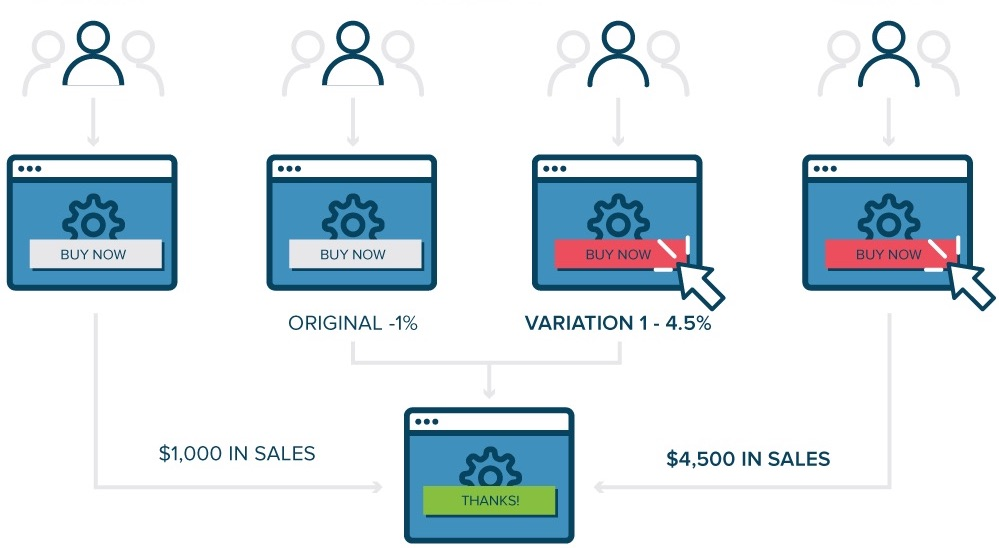
\includegraphics[height = 0.5\textwidth]{ab-testing-optimizely-2}
	\caption{A/B Test hoạt động như thế nào}
\end{figure}

Khi khách truy cập được phục vụ hoặc kiểm soát hoặc biến thể, mức độ tương tác của họ với từng trải nghiệm được đo lường và thu thập trong một bảng điều khiển và phân tích thông qua một công cụ thống kê. Sau đó, bạn có thể xác định xem việc thay đổi trải nghiệm có tác động tích cực, tiêu cực hay trung tính đến hành vi của khách truy cập hay không.

\begin{figure}[ht]
	\centering
	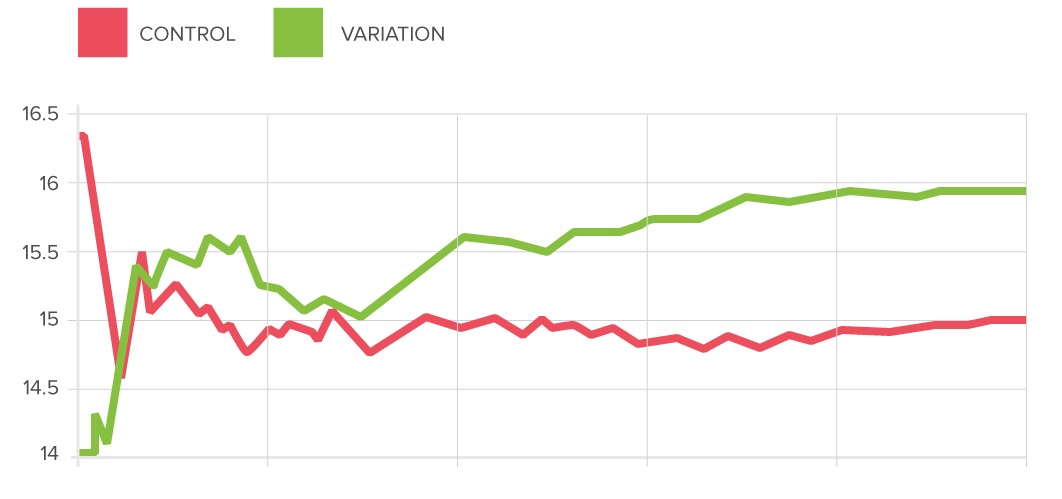
\includegraphics[height = 0.5\textwidth]{control-variation-graph-3}
	\caption{Biểu đồ so sánh kết quả các biến thể}
\end{figure}

\subsection{Ứng dụng của A/B Test}

A/B Test tăng trải nghiệm người dùng, giúp quảng cáo online thu thập được các dữ liệu lý tưởng. Họ sẽ hiểu hơn về hành vi quảng cáo nào ảnh hưởng đến người dùng để cung cấp các dịch vụ tốt nhất.

A/B Test giúp giảm tiền vào đầu tư các chiến dịch marketing. Chi phí thử nghiệm thấp nhưng hiệu quả mang về lại rất cao. Sales và marketing sẽ kết nối với nhau để tương tác hoạt động tốt hơn.

Xu hướng marketing online hiện nay đều chú trọng đến A/B Test. Chạy A/B Test cũng là một cách để kiểm tra cạnh tranh tốt hơn với các đối thủ. Để công việc kinh doanh của mình thành công bạn nên nghiên cứu về những lĩnh vực thử nghiệm này. Chúng sẽ giúp bạn thấu hiểu khách hàng, biết được hành vi của khách hàng để đưa ra các chiến lược kinh doanh quan trọng hơn.

\subsubsection{Đối với website}

Để tìm ra giao diện mà thu hút người sử dụng hơn thì chúng ta có thử nghiệm 2 phiên bản của giao diện đó, hai phiên bản sẽ khác nhau ở cách bố trí nội dung, vị trí đặt các button điều hướng, các hình ảnh, .....

\subsubsection{Đối với Email marketing}

Đã qua rồi cái thời mà đẩy hàng trăm ngàn email đi và nghĩ rằng người dùng sẽ đọc được những email của mình gửi. Các email clients ngày càng có các bộ lọc tinh xảo hơn, tống tất cả các spam email vào thùng rác. Điều quan trọng là làm thế nào để khách hàng chịu mở email của mình ra xem và tương tác với các email đó. Câu trả lời chính là A/B Test.

Bạn có thể làm A/B Test để xác định được ngày nào trong tuần tỉ lệ mở mail cao nhất, gửi thời gian nào trong ngày là tốt nhất cho nội dung của bạn, tiêu đề email nào sẽ mang lại tỉ lệ mở mail cao hơn?...

\subsubsection{Đối với quảng cáo và bán hàng}

Đối với mảng online thì A/B Test thường được dùng để đo lường hiệu quả của các mẫu quảng cáo khác nhau. Ví dụ như khi bạn viết quảng cáo Adwords cho cùng 1 nhóm từ khóa (ad group) thì bạn nên viết 2 mẫu quảng cáo khác nhau và cho chạy song song để biết mẫu quảng cáo nào hiệu quả hơn sau một thời gian chạy. Tương tự với quảng cáo cho Facebook, sử dụng các thiết kế quảng cáo khác nhau cho cùng một chiến dịch để đo lường hiệu quả sau đó chọn mẫu thiết kế nào hiệu quả hơn để chạy tiếp. Việc tối ưu hóa quảng cáo thường xuyên bằng cách test các lựa chọn khác nhau sẽ giúp bạn liên tục cải thiện được tỷ lệ chuyển đổi và giúp quảng cáo chạy ngày càng hiệu quả hơn.

Đối với mảng offline thì A/B Test thường có thể được dùng để đánh giá hiệu quả của các kênh quảng cáo như báo giấy, tờ rơi, billboard… Chẳng hạn bằng cách sử dụng các mã coupon khác nhau cho từng mẫu quảng cáo trên báo, mẫu tờ rời, hoặc billboard, nhà quảng cáo có thể nắm được mẫu quảng cáo nào hiệu quả hơn thông qua việc có nhiều người sử dụng mã coupon nào hơn.

\subsubsection{Đối với ứng dụng di động}

A/B Test cũng được ứng dụng trong việc phát triển ứng dụng di động và tương tự như website, chủ yếu nhằm cải thiện UI/UX của sản phẩm.

Với các ứng dụng điện thoại di động thì việc tiến hành test thường khó khăn hơn nhiều cả về mặt kỹ thuật lẫn về hành vi người dùng.

Về mặt kỹ thuật thì để tiến hành test, thì phiên bản ứng dụng cần được cập nhật, được duyệt bởi AppStore hay Google Play rồi mới đến với người dùng do đó tốn nhiều thời gian hơn.

Về phương diện hành vi người dùng, không phải ai cũng sẽ cập nhật ngay phiên bản mới và trải nghiệm người dùng trên điện thoại di động hoàn toàn khác so với trên web.

\subsection{Quy trình thử nghiệm A/B}

Sau đây là khung thử nghiệm A/B mà có thể sử dụng để bắt đầu chạy thử nghiệm:

\begin{itemize}
	\bfitem {Thu thập dữ liệu}{Các phân tích của bạn thường sẽ cung cấp thông tin chi tiết về nơi bạn có thể bắt đầu tối ưu hóa. Nó hữu ích để bắt đầu với các khu vực có lưu lượng truy cập cao trên trang web hoặc ứng dụng của bạn để cho phép bạn thu thập dữ liệu nhanh hơn. Tìm kiếm các trang có tỷ lệ chuyển đổi thấp hoặc tỷ lệ rớt mạng cao có thể được cải thiện.}
	\bfitem {Xác định mục tiêu}{Mục tiêu chuyển đổi của bạn là số liệu mà bạn đang sử dụng để xác định xem biến thể có thành công hơn phiên bản gốc hay không. Mục tiêu có thể là bất cứ điều gì từ việc nhấp vào nút hoặc liên kết đến việc mua sản phẩm và đăng ký e-mail.}
	\bfitem {Tạo giả thuyết}{ Khi bạn đã xác định được mục tiêu, bạn có thể bắt đầu tạo ra các ý tưởng và giả thuyết thử nghiệm A/B để biết lý do tại sao bạn cho rằng chúng sẽ tốt hơn phiên bản hiện tại. Khi bạn đã có danh sách các ý tưởng, hãy sắp xếp thứ tự ưu tiên cho chúng về tác động dự kiến và mức độ khó thực hiện.}
	\bfitem {Tạo các biến thể}{Sử dụng phần mềm thử nghiệm A/B của bạn (như Optimizely), thực hiện các thay đổi mong muốn đối với một phần tử của trang web hoặc trải nghiệm ứng dụng dành cho thiết bị di động của bạn. Điều này có thể là thay đổi màu của nút, hoán đổi thứ tự của các phần tử trên trang, ẩn các phần tử điều hướng hoặc một cái gì đó hoàn toàn tùy chỉnh. Nhiều công cụ kiểm tra A/B hàng đầu có trình chỉnh sửa trực quan sẽ giúp những thay đổi này trở nên dễ dàng. Đảm bảo QA thử nghiệm của bạn để đảm bảo thử nghiệm hoạt động như mong đợi.}
	\bfitem {Chạy thử nghiệm}{Bắt đầu thử nghiệm của bạn và đợi khách tham gia! Tại thời điểm này, khách truy cập vào trang web hoặc ứng dụng của bạn sẽ được chỉ định ngẫu nhiên cho quyền kiểm soát hoặc biến thể trải nghiệm của bạn. Tương tác của họ với từng trải nghiệm được đo lường, tính toán và so sánh để xác định cách mỗi trải nghiệm hoạt động.}
	\bfitem {Phân tích kết quả}{Sau khi thử nghiệm của bạn hoàn tất, đã đến lúc phân tích kết quả. Phần mềm thử nghiệm A/B của bạn sẽ trình bày dữ liệu từ thử nghiệm và cho bạn thấy sự khác biệt giữa hai phiên bản trang của bạn hoạt động như thế nào và liệu có sự khác biệt có ý nghĩa thống kê hay không.}
\end{itemize}

\begin{figure}[ht]
	\centering
	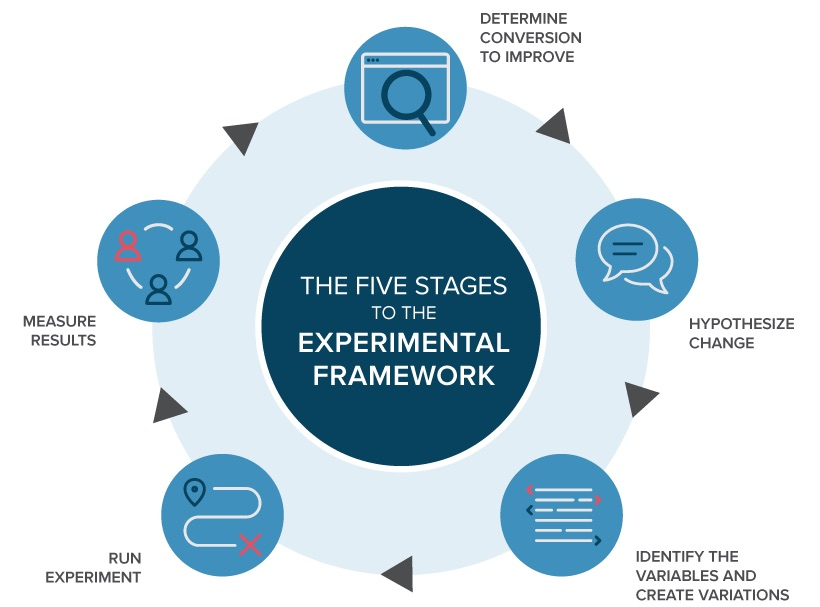
\includegraphics[height = 0.5\textwidth]{ab-testing-process-6}
	\caption{Quy trình thử nghiệm A/B}
\end{figure}

\section{Thông số của A/B Test trong Quảng Cáo}

\subsection{Tỷ lệ chuyển đổi (Conversion Rate)}

Hiểu một cách đơn giản, tỷ lệ chuyển đổi chính là tỷ lệ người truy cập vào website đã thực hiện hành động bạn mong muốn (click vào một trang quảng cáo, mua hàng, hay điền form khảo sát,....) trên tổng số lượt truy cập vào website

\begin{displaymath}
	CR = \frac{Conversions}{Clicks} * 100\%
\end{displaymath}

Lấy một ví dụ đơn giản như: Bạn có một website bán hàng, bạn muốn có thật nhiều người mua hàng trên website của bạn. Hôm nay website của bạn có 200 lượt truy cập trong đó có 5 lượt mua hàng thông qua website của bạn, khi đó bạn sẽ có con số về tỷ lệ chuyển đổi là $CR = (5/200) * 100\% = 2,5\%$. Việc của bạn là phải có các chiến lược để con số này càng cao càng tốt.

Tỷ lệ chuyển đổi tương tự như chỉ số doanh thu tăng lên vì trong thương mại điện tử, một chuyển đổi tương đương với một lần bán hàng. Tuy nhiên, việc đếm số lượng bán hàng khác với tính toán doanh thu: doanh thu cao hơn không cho thấy hoạt động tăng lên bởi vì nó dựa trên lợi nhuận chứ không chỉ dựa trên số lượng bán hàng. Biên lợi nhuận lớn có thể làm sai lệch kết quả; ví dụ, một lần bán thêm duy nhất với tỷ suất lợi nhuận lớn có thể cho thấy doanh thu tăng lên. Việc tính doanh số bán hàng đơn giản và rõ ràng hơn, nhưng điểm mạnh của nó cũng chứa một điểm yếu, như bạn sẽ thấy ở phần sau.

Lợi ích của việc sử dụng chuyển đổi làm phép đo là nó được tính ở quy mô nhỏ hơn: tìm kiếm. Do số lượng tìm kiếm dao động nhanh hơn số lượng chuyển đổi (khách hàng chuyển đổi ít thường xuyên hơn nhiều so với số lượng họ tìm kiếm), nên tỷ lệ tìm kiếm trên chuyển đổi có thể thay đổi nhanh chóng nếu khách hàng chuyển đổi thường xuyên hơn. Do đó, chuyển đổi có thể phát hiện các sửa đổi hệ thống dễ dàng hơn.

Do đó, tỷ lệ chuyển đổi ít mang tính định hướng hơn so với doanh thu nhưng có thể được phát hiện nhanh chóng - tức là tỷ lệ này nhạy cảm hơn. Thuộc tính này thích hợp hơn cho thử nghiệm A/B vì nó đạt được mức ý nghĩa nhanh hơn. Điều đó nói rằng, chuyển đổi không phải là một hình thức đo lường hoàn hảo vì nó coi tất cả doanh số bán hàng là bình đẳng, không mang lại giá trị kinh doanh giống nhau do tăng doanh thu.
\begin{figure}[ht]
	\centering
	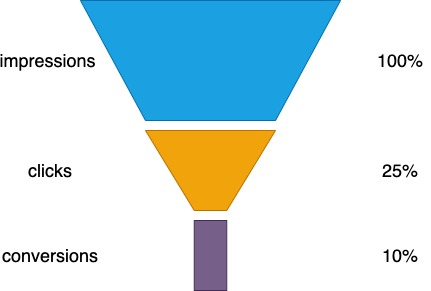
\includegraphics[height = 0.5\textwidth]{conversions}
	\caption{Conversions}
\end{figure}

\subsection{Tỷ lệ click (CTR)}

CTR là tỷ lệ cho biết tần suất những người xem quảng cáo hoặc danh sách sản phẩm sẽ nhấp vào quảng cáo hoặc danh sách sản phẩm miễn phí của bạn. Tỷ lệ nhấp (CTR) có thể được sử dụng để đánh giá mức độ hoạt động của các từ khóa và quảng cáo cũng như danh sách miễn phí của bạn.

CTR là số nhấp chuột mà quảng cáo của bạn nhận được chia cho số lần quảng cáo của bạn được hiển thị: nhấp chuột ÷ hiển thị = CTR. Ví dụ: nếu bạn có 5 nhấp chuột và 100 hiển thị, thì CTR của bạn sẽ là 5%.

\begin{displaymath}
	CTR = \frac{Clicks}{Impressions} * 100\%
\end{displaymath}

Mỗi quảng cáo, danh sách và từ khóa của bạn có CTR riêng mà bạn có thể thấy được liệt kê trong tài khoản của mình.

CTR cao là một dấu hiệu tốt cho thấy người dùng thấy quảng cáo và danh sách của bạn hữu ích và có liên quan. CTR cũng đóng góp vào CTR dự kiến của từ khóa của bạn, là một thành phần của Xếp hạng quảng cáo. Lưu ý rằng CTR tốt có liên quan đến những gì bạn đang quảng cáo và trên mạng nào.

Bạn có thể sử dụng CTR để đánh giá những quảng cáo, danh sách và từ khóa nào thành công với bạn và những quảng cáo nào cần được cải thiện. Từ khóa, quảng cáo và danh sách của bạn càng liên quan đến nhau và với doanh nghiệp của bạn, thì càng có nhiều khả năng người dùng nhấp vào quảng cáo hoặc danh sách của bạn sau khi tìm kiếm trên cụm từ khóa của bạn.

\section{Cấu trúc của A/B Test}

Một A/B Test được chia làm thành nhiều tầng lớp.  Mỗi tầng lớp đều có ý nghĩa riêng và được chia ra để có thể phục vụ cho logic business phức tạp.

\begin{figure}[ht]
	\centering
	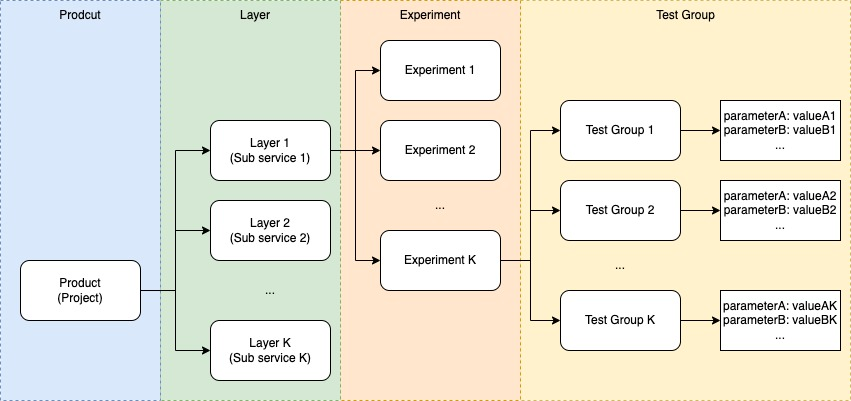
\includegraphics[height = 0.5\textwidth]{overview-ab-testing}
	\caption{Tổng quan của một A/B Test}
\end{figure}

\subsection{Product}

Product là thực thể cao nhất trong một A/B Test. Mỗi product thường đại diện cho một tập thể lớn. Mỗi team thường có nhiều bộ phận cho các lĩnh vực khác nhau, mỗi bộ phận sẽ thường có một hoặc nhiều Product.

Mỗi Product được chia ra để tách biệt các A/B Test giữa các team khác nhau. A/B Test thuộc hai Product khác nhau sẽ không liên quan gì đến nhau, không để so sánh được cùng với nhau.

\begin{figure}[ht]
	\centering
	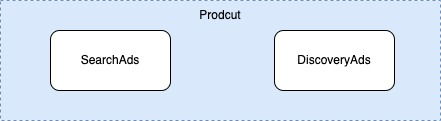
\includegraphics[width = 1\textwidth]{product}
	\caption{Product}
\end{figure}

Ví dụ: trong phòng quảng cáo thì sẽ có hai bộ phận lớn là quảng cáo tìm kiếm và quảng cáo gợi ý. Mỗi bộ phận sẽ có 2 product khác nhau để khi thực hiện A/B Test không ảnh hưởng lẫn nhau.

\subsection{Layer}

Layer là thực thể thức hai đứng sau thực thể Product. Một Product có thể có nhiều Layer. Mỗi Layer đại diện cho một logic nhỏ hơn của Product đấy. Mỗi layer sẽ có 100\% lượng truy cập.

Ví dụ: trong mobile app có thể có 2 layer là layer giao diện cài đặt hay layer giao diện chơi game.

Ngoài ra, với mỗi layer, có thể cài đặt layer này sử dụng một cơ số để phân chia lượng truy cập. Các cơ số có thể là:

\begin{itemize}
	\bfitem {request\_id}{sử dụng request\_id để phân chia truy cập.}
	\bfitem {user\_id}{sử dụng user\_id để phân chia truy cập.}
	\bfitem {request\_id và user\_id}{sử dụng cả request\_id và user\_id để phân chia truy cập.}
\end{itemize}

Khi một truy cập được thông qua, truy cập đó sẽ đi qua từng Layer. Với mỗi layer, nó sẽ sử dụng cơ số để quyết định xem layer này sẽ sử dụng A/B Test hay thí nghiệm nào.

\begin{figure}[ht]
	\centering
	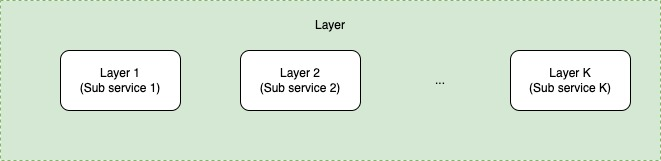
\includegraphics[width = 1\textwidth]{layer}
	\caption{Layer}
\end{figure}

\subsection{Experiment}

Experiment là thực thể tiếp theo đứng dưới một layer. Một experiment chính là một thí nghiệm mà được tạo ra để thử nghiệm một mô hình tính toán mới. Ví dụ: thử nghiệm thuật toán A mới để tính toán giá cả, thử nghiệm giao dịch màu mới để tăng trải nghiệm người dùng, v.v.

Mỗi experiment sẽ thuộc một Layer và chiếm một tỉ lệ phần trăm truy cập của layer đó. Một layer có thể có nhiều experiment. Ví dụ: layer tính toán giá cả sẽ có hai thí nghiệm thử nghiệm hai thuật toán A và B, mỗi thuật toán có 10\% lượng truy cập để đánh giá.

Như vậy, với mỗi layer, khi một try cập đi đến, nó sẽ sử dụng không hoặc một experiment.

\begin{figure}[ht]
	\centering
	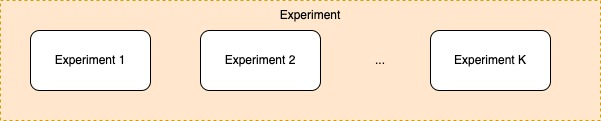
\includegraphics[width = 1\textwidth]{experiment}
	\caption{Experiment}
\end{figure}

\subsection{Test Group}

Test Group là thực thể nhỏ nhất trong một A/B Test. Test Group đại diện cho một biến thể của một Experiment. Ví dụ khi sử dụng thuật toán A để tính toán giá cả của sản phẩm, thuật toán A có thể sử dụng hai chỉ số khác nhau để tính toán tương ứng với hai test group khác nhau.

Khi thực hiện một Experiment, mỗi Test Group sẽ có một lượng truy cập giống nhau và kết quả sẽ được so sánh giữa hai Test Group. Ví dụ trong thuật toán A, hai biến thể X và Y sẽ có một biến thể mang lại kết quả tốt hơn khi so sánh với nhau.

\begin{figure}[ht]
	\centering
	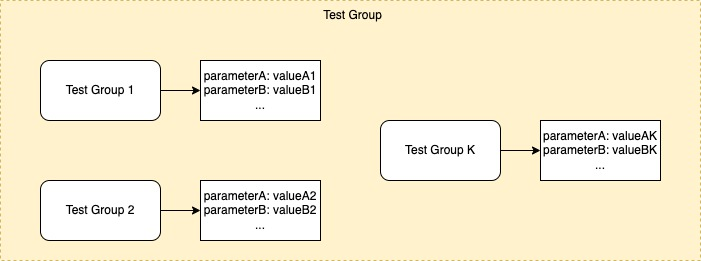
\includegraphics[width = 1\textwidth]{test-group}
	\caption{Test Group}
\end{figure}

\section{Công nghệ thực hiện}

\subsection{Golang}

\begin{figure}[ht]
	\centering
	
\includegraphics[height = 0.3\textwidth]{golang}
	\caption{Golang}
\end{figure}

Golang còn được gọi là Go là một ngôn ngữ lập trình open-source, compiled và statically-typed do Google phát triển.

Go là một ngôn ngữ lập trình đa năng với cú pháp đơn giản và một thư viện tiêu chuẩn mạnh mẽ. Go cải thiện các khái niệm như lập trình mệnh lệnh và hướng đối tượng và do đó đơn giản hóa môi trường làm việc cho các lập trình viên.

% \subsubsection{Lịch sử của Golang}
%
% Ngôn ngữ lập trình Go ra đời bởi vì mọi thứ trở nên phức tạp hơn nhiều trong codebases của Google.
%
% Nó được thiết kế bởi Robert Griesemer, Rob Pike và Ken Thompson, những người được cho là có chung sở thích với C++.
%
% Go được công bố ra mắt công chúng vào năm 2009, và nó được làm mã nguồn mở vào năm 2012 khi phiên bản đầu tiên của nó, 1.0, được phát hành.
%
% Go nhanh chóng trở nên phổ biến và trở thành lựa chọn đầu tiên của nhiều nhà phát triển do tính đơn giản, dễ đọc, hiệu quả và tính đồng thời của nó. Đồng thời có nghĩa là nó có thể chạy nhiều tác vụ cùng một lúc.
%
% Go được sử dụng để lập trình phía máy chủ, phát triển trò chơi, lập trình dựa trên đám mây và thậm chí cả Khoa học dữ liệu. Nó cũng phổ biến để tạo các công cụ dòng lệnh.
%
% Ngày nay, nhiều gã khổng lồ công nghệ sử dụng Go như Google, Netflix, Twitch, Ethereum, Dropbox, Kubernetes, Docker, Heroku, v.v.
%
% Không có gì ngạc nhiên khi những người như Kubernetes, Docker và Heroku đang sử dụng cờ vây vì cloud-based programming là một trong những lý do chính khiến Go được thiết kế.
%
% \begin{figure}[ht]
% 	\centering
% 	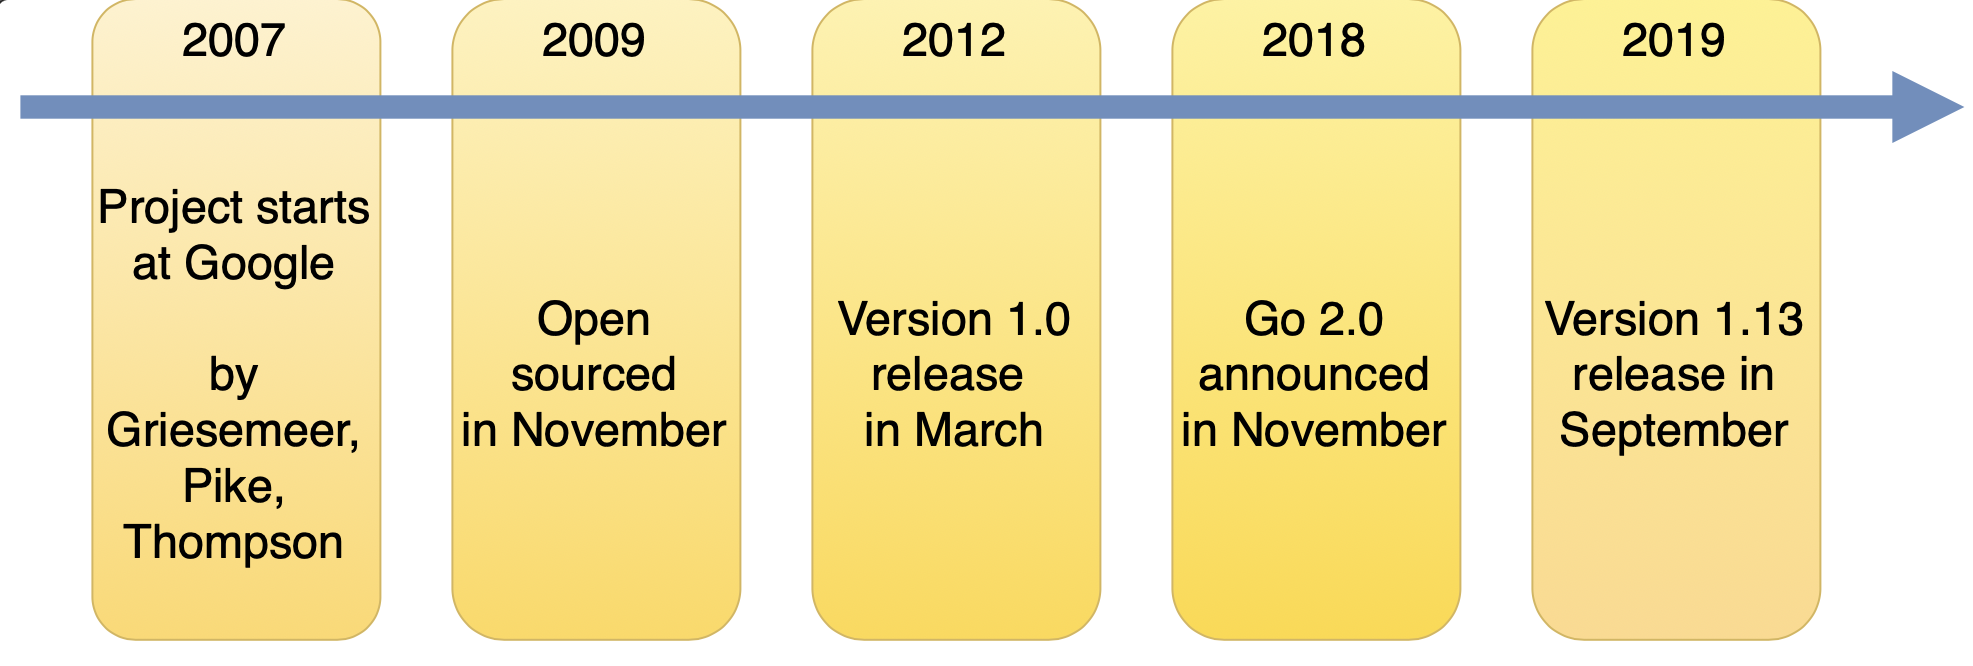
\includegraphics[height = 0.3\textwidth]{golang-history-timeline}
% 	\caption{Lịch sử của Golang}
% \end{figure}

\subsubsection{Ưu điểm của Golang}

\begin{itemize}
	\bfitem {Cú pháp đơn giản}{Go có cú pháp ngắn gọn và đơn giản giúp viết mã dễ đọc và dễ bảo trì.}
	\bfitem {Ngôn ngữ biên dịch}{}
	\bfitem {Liên kết tĩnh}{Trình biên dịch hỗ trợ liên kết tĩnh có nghĩa là bạn có thể liên kết tĩnh dự án của mình thành một tệp nhị phân lớn và sau đó chỉ cần triển khai nó lên máy chủ.}
	\bfitem {Mã nguồn mở}{Go là mã nguồn mở nên bạn có thể đọc mã nguồn và đóng góp vào kho lưu trữ.}
	\bfitem {Ngôn ngữ Strong và Statically Type}{Strong có nghĩa là sau khi bạn tạo một số biến bằng cách sử dụng một số kiểu dữ liệu thì đối với toàn bộ ứng dụng, nó sẽ vẫn là kiểu dữ liệu đấy. Statically Type là tất cả các biến phải xác định tại thời điểm biên dịch.}
	\bfitem {Cộng đồng mạnh}{Golang có một cộng đồng tuyệt vời để theo dõi vấn đề và giải pháp.}
	\bfitem {Biên dịch nhanh}{Golang sẽ chỉ bao gồm các gói sẽ nhập trực tiếp trong mã.}
	\bfitem {Garbage Collector}{Đó là một tính năng chính của Go. Go vượt trội trong việc cung cấp nhiều quyền kiểm soát đối với việc phân bổ bộ nhớ và đã giảm đáng kể độ trễ trong các phiên bản gần đây nhất của Garbage Collector.}
	\bfitem {Concurrency tích hợp}{Go có tính năng concurrency được tích hợp sẵn. Sử dụng Go Routines và các kênh, bạn có thể xử lý đồng thời các tác vụ rất dễ dàng và hiệu quả.}
	\begin{figure}[ht]
		\centering
		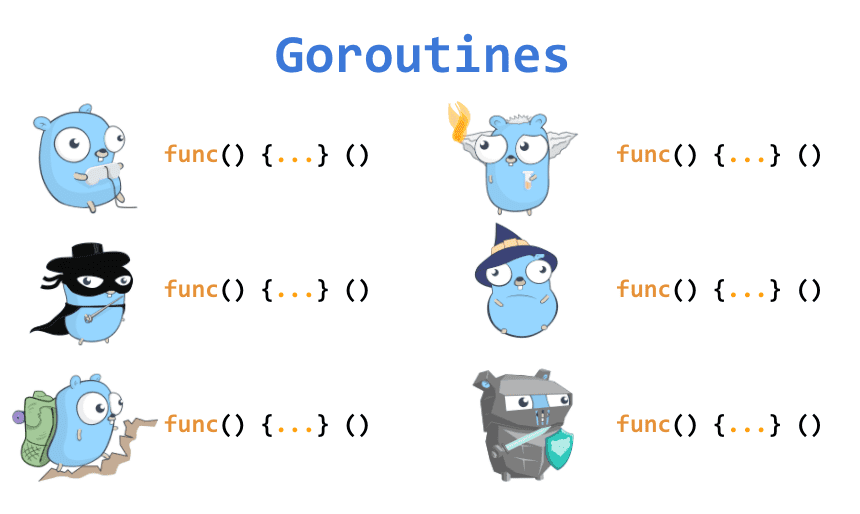
\includegraphics[height = 0.3\textwidth]{goroutines}
		\caption{Goroutine}
	\end{figure}
	\begin{figure}[ht]
		\centering
		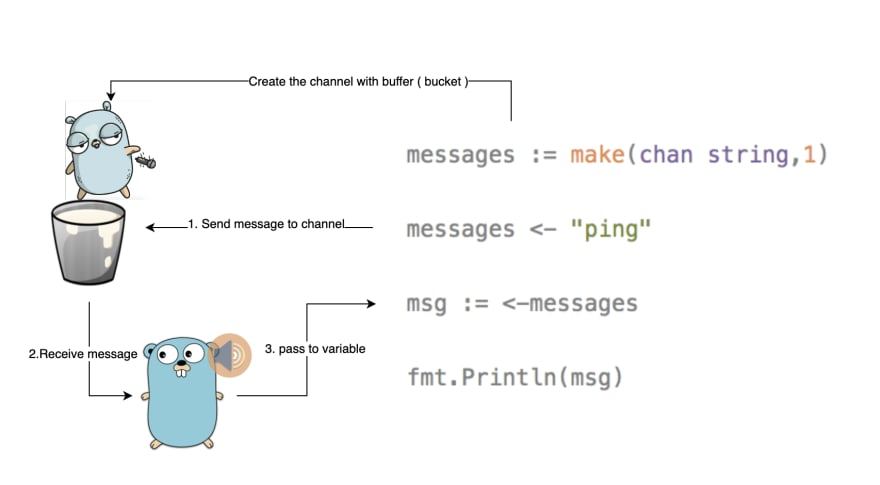
\includegraphics[height = 0.3\textwidth]{channel}
		\caption{Channel}
	\end{figure}
\end{itemize}

\subsubsection{Ứng dụng của Golang}

\begin{itemize}
	\bfitem{Dịch vụ đám mây \& mạng}{Go giúp các doanh nghiệp xây dựng và mở rộng quy mô hệ thống điện toán đám mây. Khi các ứng dụng và quá trình xử lý chuyển sang đám mây, đồng thời trở thành một vấn đề rất lớn. Về bản chất, các hệ thống điện toán đám mây chia sẻ và mở rộng quy mô tài nguyên. Điều phối quyền truy cập vào các tài nguyên được chia sẻ là một vấn đề ảnh hưởng đến mọi quá trình xử lý ứng dụng trên đám mây và yêu cầu ngôn ngữ lập trình “hướng đến phát triển các ứng dụng đồng thời có độ tin cậy cao”.}
	\bfitem {Command-line Interfaces (CLIs)}{Giao diện dòng lệnh (CLI), không giống như giao diện người dùng đồ họa (GUI), chỉ ở dạng văn bản. Các ứng dụng cơ sở hạ tầng và đám mây chủ yếu dựa trên CLI do khả năng tự động hóa và điều khiển từ xa dễ dàng.}
	\bfitem {Web Development}{Go được thiết kế để cho phép các nhà phát triển nhanh chóng phát triển các ứng dụng web có khả năng mở rộng và bảo mật. Go đi kèm với một máy chủ web dễ sử dụng, an toàn và hiệu quả và bao gồm thư viện tạo khuôn mẫu web riêng. Go có hỗ trợ tuyệt vời cho tất cả các công nghệ mới nhất từ HTTP / 2, cơ sở dữ liệu như MySQL, MongoDB và ElasticSearch, cho đến các tiêu chuẩn mã hóa mới nhất bao gồm TLS 1.3. Các ứng dụng web của Go chạy nguyên bản trên Google App Engine và Google Cloud Run (để dễ dàng mở rộng quy mô) hoặc trên bất kỳ môi trường, đám mây hoặc hệ điều hành nào nhờ tính di động cực cao của Go.}
	\bfitem {Development Operations \& Site Reliability Engineering}{Thời gian khởi động và xây dựng nhanh. Thư viện tiêu chuẩn mở rộng của Go — bao gồm các gói cho các nhu cầu thông thường như HTTP, I / O tệp, thời gian, biểu thức chính quy, thực thi và các định dạng JSON / CSV — cho phép DevOps / SRE đi đúng vào logic kinh doanh của họ. Ngoài ra, hệ thống kiểu tĩnh và xử lý lỗi rõ ràng của Go giúp các tập lệnh nhỏ thậm chí còn mạnh mẽ hơn.}
\end{itemize}

\subsection{React}

\begin{figure}[ht]
	\centering
	
\includegraphics[height = 0.3\textwidth]{react}
	\caption{React}
\end{figure}

\subsubsection{React là gì}

React (còn được gọi là React.js hoặc ReactJS) là một thư viện JavaScript front-end mã nguồn mở và miễn phí để xây dựng giao diện người dùng dựa trên các thành phần UI. Nó được duy trì bởi Meta (trước đây là Facebook) và một cộng đồng các nhà phát triển và công ty cá nhân. React có thể được sử dụng làm cơ sở để phát triển các single-page, ứng dụng di động hoặc ứng dụng web với các framework như Next.js.

Tuy nhiên, React chỉ quan tâm đến việc quản lý trạng thái và hiển thị trạng thái đó cho DOM, vì vậy việc tạo các ứng dụng React thường yêu cầu sử dụng các thư viện bổ sung để định tuyến, cũng như một số chức năng phía client.

\subsubsection{Đặc trưng của React}

\textbf{Declarative}

React giúp tạo giao diện người dùng tương tác dễ dàng hơn. Thiết kế các khung nhìn đơn giản cho từng trạng thái trong ứng dụng của bạn và React sẽ cập nhật và hiển thị các thành phần phù hợp một cách hiệu quả khi dữ liệu của bạn thay đổi.

Chế độ xem Declarative làm cho code của bạn dễ đoán hơn và dễ debug hơn.

\textbf{Component-Based}

Xây dựng các thành phần được đóng gói quản lý trạng thái của riêng chúng, sau đó biên soạn chúng để tạo giao diện người dùng phức tạp.

Vì logic thành phần được viết bằng JavaScript thay vì các mẫu, bạn có thể dễ dàng chuyển dữ liệu phong phú thông qua ứng dụng của mình và giữ trạng thái không nằm trong DOM.

\textbf{Learn Once, Write Anywhere}

Chúng tôi không đưa ra giả định về phần còn lại của nền tảng công nghệ của bạn, vì vậy bạn có thể phát triển các tính năng mới trong React mà không cần viết lại mã hiện có.

React cũng có thể render trên server bằng Node và compile ra các ứng dụng di động bằng React Native.

\textbf{Virtual DOM}

\begin{figure}[ht]
	\centering
	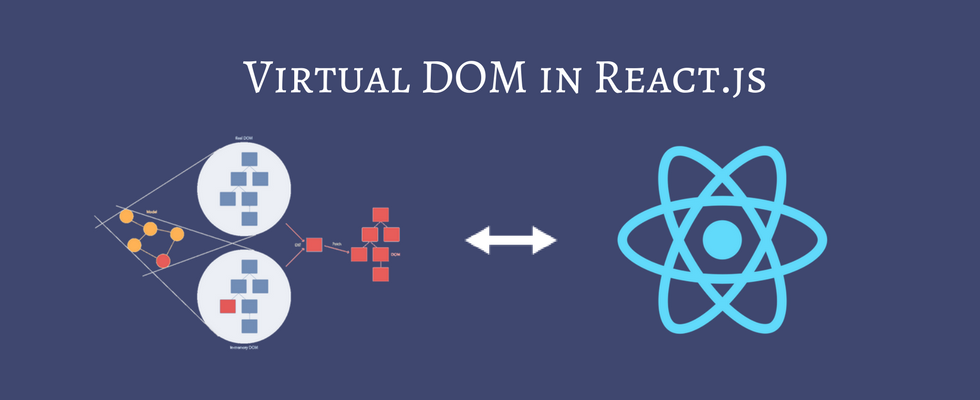
\includegraphics[height = 0.3\textwidth]{virtual-dom}
	\caption{Virtual DOM}
\end{figure}

Những Framework sử dụng Virtual-DOM như ReactJS khi Virtual-DOM thay đổi, chúng ta không cần thao tác trực tiếp với DOM trên View mà vẫn phản ánh được sự thay đổi đó. Do Virtual-DOM vừa đóng vai trò là Model, vừa đóng vai trò là View nên mọi sự thay đổi trên Model đã kéo theo sự thay đổi trên View và ngược lại. Có nghĩa là mặc dù chúng ta không tác động trực tiếp vào các phần tử DOM ở View nhưng vẫn thực hiện được cơ chế Data-binding. Điều này làm cho tốc độ ứng dụng tăng lên đáng kể – môt lợi thế không thể tuyệt vời hơn khi sử dụng Virtula-DOM.

\subsubsection{Ứng dụng của React}

\subsection{Redis}

\begin{figure}[ht]
	\centering
	
\includegraphics[height = 0.3\textwidth]{redis}
	\caption{Redis}
\end{figure}

\subsubsection{Redis là gì}

Redis, viết tắt của Remote Dictionary Server, là một kho lưu trữ dữ liệu key-value, mã nguồn mở, in-memeory và nhanh chóng. Dự án bắt đầu khi Salvatore Sanfilippo, nhà phát triển ban đầu của Redis, muốn cải thiện khả năng mở rộng của công ty khởi nghiệp của mình. Từ đó, anh phát triển Redis, hiện được sử dụng làm cơ sở dữ liệu, bộ nhớ đệm, message broker và hàng đợi.

Redis cung cấp thời gian phản hồi dưới mili giây, cho phép hàng triệu yêu cầu mỗi giây cho các ứng dụng thời gian thực trong các ngành như trò chơi, công nghệ quảng cáo, dịch vụ tài chính, chăm sóc sức khỏe và IoT. Ngày nay, Redis là một trong những engine mã nguồn mở phổ biến nhất hiện nay, được Stack Overflow đặt tên là cơ sở dữ liệu "Được yêu thích nhất" trong 5 năm liên tiếp. Do hiệu suất nhanh, Redis là một lựa chọn phổ biến cho bộ nhớ đệm, quản lý phiên, chơi trò chơi, bảng xếp hạng, phân tích thời gian thực, không gian địa lý, gọi xe, trò chuyện / nhắn tin, phát trực tuyến phương tiện và ứng dụng pub / sub.

\subsubsection{Tính năng của Redis}

\begin{figure}[ht]
	\centering
	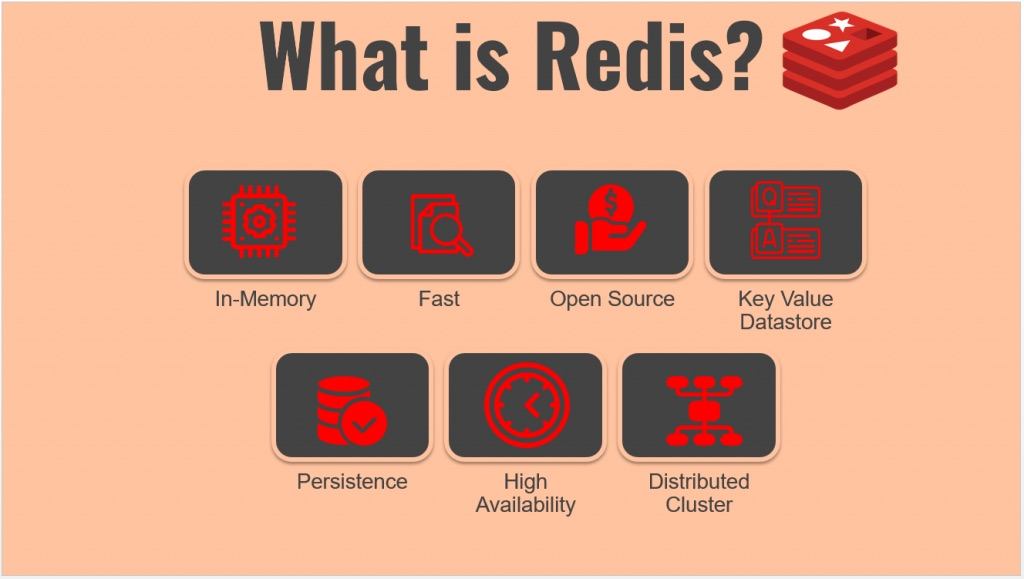
\includegraphics[width = 1\textwidth]{redis-features}
	\caption{Tính năng của Redis}
\end{figure}

\textbf{Performance}

Tất cả dữ liệu Redis nằm trong bộ nhớ, cho phép truy cập dữ liệu có độ trễ thấp và thông lượng cao. Không giống như cơ sở dữ liệu truyền thống, kho lưu trữ dữ liệu trong bộ nhớ không yêu cầu chuyển tới đĩa, giảm độ trễ của động cơ xuống micro giây. Do đó, các kho lưu trữ dữ liệu trong bộ nhớ có thể hỗ trợ nhiều thao tác hơn và thời gian phản hồi nhanh hơn. Kết quả là mang lại hiệu suất cực nhanh với các thao tác đọc và ghi trung bình chỉ mất chưa đến một phần nghìn giây và hỗ trợ hàng triệu thao tác mỗi giây.

\textbf{Cấu trúc dữ liệu linh hoạt}

Không giống như các kho dữ liệu khóa-giá trị khác cung cấp cấu trúc dữ liệu hạn chế, Redis có rất nhiều cấu trúc dữ liệu để đáp ứng nhu cầu ứng dụng của bạn. Các kiểu dữ liệu của Redis bao gồm:

\begin{figure}[ht]
	\centering
	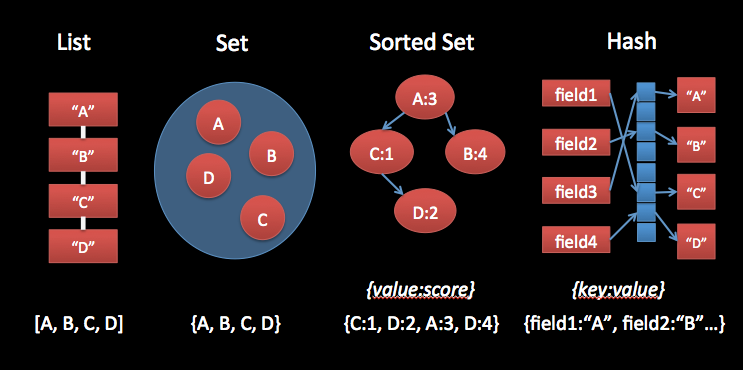
\includegraphics[width = 1\textwidth]{redis-data-structures}
	\caption{Cấu trúc dữ liệu của Redis}
\end{figure}

\begin{itemize}
	\bfitem{Strings}{dữ liệu văn bản hoặc dữ liệu nhị phân có kích thước lên đến 512MB}
	\bfitem{Lists}{tập hợp các Chuỗi theo thứ tự chúng được thêm vào}
	\bfitem{Sets}{một tập hợp các chuỗi không có thứ tự với khả năng giao nhau, kết hợp và khác các loại Bộ khác}
	\bfitem{Sorted Sets }{Các bộ được sắp xếp theo một giá trị}
	\bfitem{Hashes}{một cấu trúc dữ liệu để lưu trữ danh sách các trường và giá trị}
	\bfitem{Bitmap}{một kiểu dữ liệu cung cấp các hoạt động ở mức bit}
	\bfitem{HyperLogLogs}{cấu trúc dữ liệu xác suất để ước tính các mục duy nhất trong tập dữ liệu}
	\bfitem{Streams}{cấu trúc dữ liệu nhật ký Hàng đợi tin nhắn}
	\bfitem{Geospatial}{mục nhập dựa trên kinh độ / vĩ độ Bản đồ, "lân cận"}
	\bfitem{JSON}{một đối tượng lồng nhau, bán cấu trúc của các giá trị được đặt tên hỗ trợ số, chuỗi, Boolean, mảng và các đối tượng khác}
\end{itemize}

\textbf{Đơn giản và dễ sử dụng}

Redis cho phép bạn viết mã phức tạp truyền thống với ít dòng hơn, đơn giản hơn. Với Redis, bạn viết ít dòng mã hơn để lưu trữ, truy cập và sử dụng dữ liệu trong các ứng dụng của mình. Sự khác biệt là các nhà phát triển sử dụng Redis có thể sử dụng cấu trúc lệnh đơn giản trái ngược với các ngôn ngữ truy vấn của cơ sở dữ liệu truyền thống. Ví dụ: bạn có thể sử dụng cấu trúc dữ liệu băm Redis để di chuyển dữ liệu đến kho dữ liệu chỉ với một dòng mã. Một tác vụ tương tự trên kho dữ liệu không có cấu trúc dữ liệu băm sẽ yêu cầu nhiều dòng mã để chuyển đổi từ định dạng này sang định dạng khác. Redis đi kèm với cấu trúc dữ liệu gốc và nhiều tùy chọn để thao tác và tương tác với dữ liệu của bạn. Hơn một trăm ứng dụng khách mã nguồn mở có sẵn cho các nhà phát triển Redis. Các ngôn ngữ được hỗ trợ bao gồm Java, Python, PHP, C, C++, C\#, JavaScript, Node.js, Ruby, R, Go và nhiều ngôn ngữ khác.

\textbf{Nhân rộng và bền bỉ}

Redis sử dụng kiến trúc bản sao chính và hỗ trợ sao chép không đồng bộ, nơi dữ liệu có thể được sao chép sang nhiều máy chủ bản sao. Điều này cung cấp hiệu suất đọc được cải thiện (vì các yêu cầu có thể được phân chia giữa các máy chủ) và khôi phục nhanh hơn khi máy chủ chính gặp sự cố. Để bền bỉ, Redis hỗ trợ sao lưu theo thời gian (sao chép tập dữ liệu Redis vào đĩa).

Redis không được xây dựng để trở thành một cơ sở dữ liệu bền và nhất quán. Nếu bạn cần một cơ sở dữ liệu bền, tương thích với Redis, hãy xem xét Amazon MemoryDB cho Redis. Bởi vì MemoryDB sử dụng nhật ký giao dịch lâu dài để lưu trữ dữ liệu trên nhiều Vùng khả dụng (AZ), bạn có thể sử dụng nó làm cơ sở dữ liệu chính của mình. MemoryDB được xây dựng có mục đích cho phép các nhà phát triển sử dụng API Redis mà không phải lo lắng về việc quản lý bộ nhớ cache, cơ sở dữ liệu riêng biệt hoặc cơ sở hạ tầng bên dưới.

\textbf{Tính khả dụng và khả năng mở rộng cao}

Redis cung cấp một kiến trúc bản sao chính trong một nút chính hoặc một cấu trúc liên kết nhóm. Điều này cho phép bạn xây dựng các giải pháp có tính khả dụng cao, cung cấp hiệu suất và độ tin cậy nhất quán. Khi bạn cần điều chỉnh kích thước cụm của mình, các tùy chọn khác nhau để mở rộng và mở rộng quy mô trong hoặc ngoài cũng có sẵn. Điều này cho phép cụm của bạn phát triển theo nhu cầu của bạn.

\textbf{Mã nguồn mở}

Redis là một dự án mã nguồn mở được hỗ trợ bởi một cộng đồng sôi động, bao gồm AWS. Không có nhà cung cấp hoặc công nghệ nào bị khóa vì Redis dựa trên các tiêu chuẩn mở, hỗ trợ các định dạng dữ liệu mở và có một tập hợp khách hàng phong phú.

\subsubsection{Ứng dụng của Redis}

\begin{figure}[ht]
	\centering
	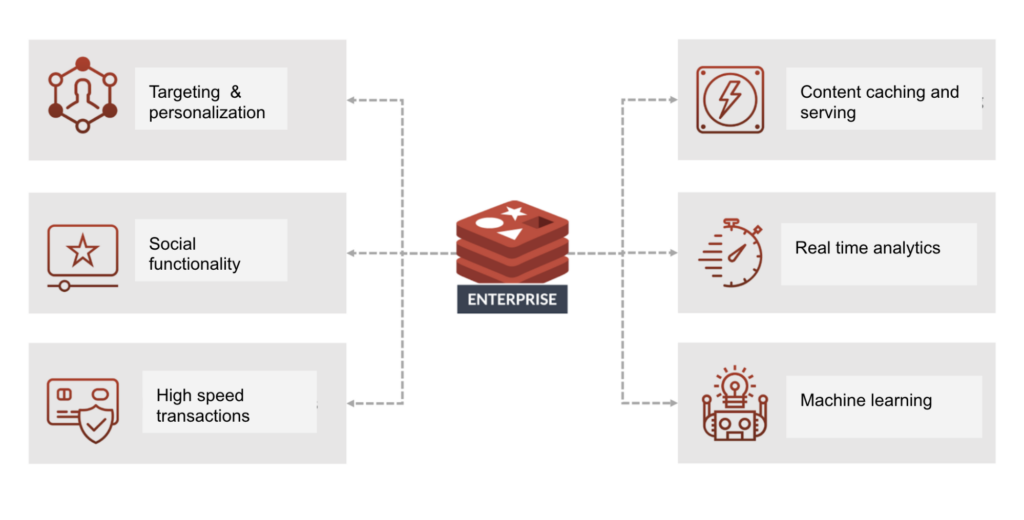
\includegraphics[width = 1\textwidth]{redis-use-cases}
	\caption{Ứng dụng của Redis}
\end{figure}

\textbf{Bộ nhớ đệm}

Redis là một lựa chọn tuyệt vời để triển khai bộ nhớ đệm trong bộ nhớ sẵn có cao để giảm độ trễ truy cập dữ liệu, tăng thông lượng và giảm tải cơ sở dữ liệu và ứng dụng NoSQL hoặc cơ sở dữ liệu quan hệ của bạn. Redis có thể phân phát các mặt hàng được yêu cầu thường xuyên ở thời gian phản hồi dưới mili giây và cho phép bạn dễ dàng mở rộng quy mô để có tải cao hơn mà không tăng phần phụ trợ tốn kém hơn. Bộ nhớ đệm kết quả truy vấn cơ sở dữ liệu, bộ nhớ đệm phiên liên tục, bộ nhớ đệm trang web và bộ nhớ đệm của các đối tượng được sử dụng thường xuyên như hình ảnh, tệp và siêu dữ liệu đều là những ví dụ phổ biến về bộ nhớ đệm với Redis.

\textbf{Trò chuyện, nhắn tin và hàng đợi}

Redis hỗ trợ Pub / Sub với tính năng so khớp mẫu và nhiều cấu trúc dữ liệu khác nhau như danh sách, tập hợp được sắp xếp và băm. Điều này cho phép Redis hỗ trợ các phòng trò chuyện hiệu suất cao, luồng bình luận trong thời gian thực, nguồn cấp dữ liệu mạng xã hội và giao tiếp liên máy chủ. Cấu trúc dữ liệu Redis List giúp dễ dàng triển khai một hàng đợi nhẹ. Danh sách cung cấp các hoạt động nguyên tử cũng như khả năng chặn, làm cho chúng phù hợp với nhiều ứng dụng khác nhau yêu cầu trình môi giới thông điệp đáng tin cậy hoặc danh sách vòng tròn.

\textbf{Bảng thành tích}

Redis là một lựa chọn phổ biến trong số các nhà phát triển trò chơi đang tìm cách xây dựng bảng xếp hạng thời gian thực. Chỉ cần sử dụng cấu trúc dữ liệu Redis Sorted Set, cung cấp tính duy nhất của các phần tử trong khi vẫn duy trì danh sách được sắp xếp theo điểm số của người dùng. Việc tạo danh sách được xếp hạng theo thời gian thực cũng dễ dàng như việc cập nhật điểm của người dùng mỗi khi nó thay đổi. Bạn cũng có thể sử dụng Bộ đã sắp xếp để xử lý dữ liệu chuỗi thời gian bằng cách sử dụng dấu thời gian làm điểm số.

\textbf{Lưu trữ session}

Redis như một kho lưu trữ dữ liệu trong bộ nhớ với tính khả dụng cao và bền bỉ là lựa chọn phổ biến của các nhà phát triển ứng dụng để lưu trữ và quản lý dữ liệu phiên cho các ứng dụng quy mô internet. Redis cung cấp độ trễ dưới mili giây, quy mô và khả năng phục hồi cần thiết để quản lý dữ liệu phiên, chẳng hạn như hồ sơ người dùng, thông tin đăng nhập, trạng thái phiên và cá nhân hóa người dùng cụ thể.

\textbf{Phát trực tuyến đa phương tiện}

Redis cung cấp một kho lưu trữ dữ liệu trong bộ nhớ, nhanh chóng để cung cấp năng lượng cho các trường hợp sử dụng phát trực tiếp. Redis có thể được sử dụng để lưu trữ siêu dữ liệu về hồ sơ của người dùng và lịch sử xem, thông tin xác thực / mã thông báo cho hàng triệu người dùng và tệp kê khai để cho phép CDN truyền video tới hàng triệu người dùng thiết bị di động và máy tính để bàn cùng một lúc.

\textbf{Không gian địa lý}

Redis cung cấp các cấu trúc và toán tử dữ liệu trong bộ nhớ được xây dựng có mục đích để quản lý dữ liệu không gian địa lý theo thời gian thực ở quy mô và tốc độ. Các lệnh như GEOADD, GEODIST, GEORADIUS và GEORADIUSBYMEMBER để lưu trữ, xử lý và phân tích dữ liệu không gian địa lý trong thời gian thực giúp không gian địa lý trở nên dễ dàng và nhanh chóng với Redis. Bạn có thể sử dụng Redis để thêm các tính năng dựa trên vị trí như thời gian lái xe, khoảng cách lái xe và các điểm ưa thích vào ứng dụng của bạn.

\textbf{Học máy}

Các ứng dụng hướng dữ liệu hiện đại yêu cầu máy học để xử lý nhanh chóng một khối lượng lớn, sự đa dạng và tốc độ của dữ liệu cũng như tự động hóa việc ra quyết định. Đối với các trường hợp sử dụng như phát hiện gian lận trong trò chơi và dịch vụ tài chính, đặt giá thầu thời gian thực trong công nghệ quảng cáo và mai mối trong việc hẹn hò và chia sẻ chuyến đi, khả năng xử lý dữ liệu trực tiếp và đưa ra quyết định trong vòng hàng chục mili giây là vô cùng quan trọng. Redis cung cấp cho bạn một kho lưu trữ dữ liệu trong bộ nhớ nhanh chóng để xây dựng, đào tạo và triển khai các mô hình học máy một cách nhanh chóng.

\textbf{Phân tích thời gian thực}

Redis có thể được sử dụng với các giải pháp phát trực tuyến như Apache Kafka và Amazon Kinesis như một kho lưu trữ dữ liệu trong bộ nhớ để nhập, xử lý và phân tích dữ liệu thời gian thực với độ trễ dưới mili giây. Redis là một lựa chọn lý tưởng cho các trường hợp sử dụng phân tích thời gian thực như phân tích phương tiện truyền thông xã hội, nhắm mục tiêu quảng cáo, cá nhân hóa và IoT.

% \subsection{Domain Driven Design (DDD)}
%
% \subsubsection{Tầng Application}
%
% This layer doesn’t contain business logic. It’s the part that leads the user from one to another UI screen. It also interacts with application layers of other systems. It can perform simple validation but it contains no domain-related logic or data access. Its purpose is to organize and delegate domain objects to do their job. Moreover, it’s the only layer accessible to other bounded contexts.
%
% \subsubsection{Tầng Domain}
%
% This is where the concepts of the business domain are. This layer has all the information about the business case and the business rules. Here’s where the entities are. As we mentioned earlier, entities are a combination of data and behavior, like a user or a product.
%
% They have a unique identity guaranteed via a unique key and remains even when their attributes change. For example, in an e-commerce store, every order has a unique identifier. It has to go through several actions like confirming and shipping to be considered as an entity.
%
% On the other hand, value objects don’t have unique identifiers. They represent attributes that various entities can share. For example, this could be the same last name of different customers.
%
% This part also contains services with defined operational behavior that don’t have to be a part of any domain. However, they are still part of the business domain. The services are named according to the ubiquitous language. They shouldn’t deprive entities and value objects of their clear accountability and actions. Customers should be able to use any given service instance. The history of that instance during the lifetime of the application shouldn’t be a problem.
%
% Most importantly, the domain layer is in the center of the business application. This means that it should be separated from the rest of the layers. It shouldn’t depend on the other layers or their frameworks.
%
% \subsubsection{Tầng Infrastructure}
%
% This layer supports communication between other layers and can contain supporting libraries for the UI layer.

% \subsection{Test Driven Development (TDD)}


\chapter{KIẾN THỨC HỆ THỐNG}
\chapter{KIẾN THỨC HỆ THỐNG}

\section{Cơ sở lý thuyết của kiến trúc}

\subsection{Kiến trúc Modular}

Kiến trúc Modular là kiểu kiến trúc phần mềm cho phép quản lý sự phức tạp của một vấn đề bằng cách chia nhỏ chúng thành các Modular để dễ quản lý hơn với các nguyên tắc và mô hình. Modular là một đơn vị phần mềm không trạng thái có thể triển khai, quản lý, tái sử dụng, kết hợp lại và cung cấp giao diện ngắn gọn cho người dùng.

Khi phát triển phần mềm, khi hệ thống càng lớn thì càng cần thêm nhiều component, dẫn tới sự thay đổi nhỏ trong một component có thể ảnh hưởng tới nhiều component khác. Trong hệ thống, module là những component được phát triển bên ngoài ứng dụng. Module giao tiếp với ứng dụng thông qua entry-point.

\begin{figure}[H]
	\centering
	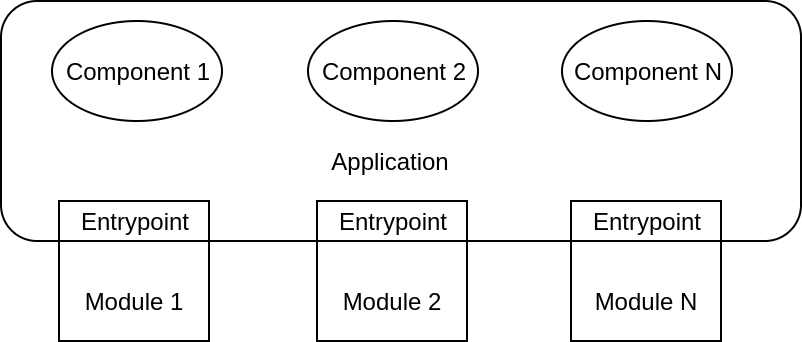
\includegraphics[width = 1\textwidth]{modules}
	\caption{Kiến trúc Modular}
\end{figure}

Sử dụng kiến trúc Modular đem lại một số lợi ích:

\begin{itemize}
	\bfitem{Tùy chỉnh}{ứng dụng có thể hoạt động thực sự khác biệt bằng cách chỉ bật / tắt một số Modular.}
	\bfitem{Ít phụ thuộc hơn}{các Modular độc lập hơn với chính ứng dụng, cho đến khi các "điểm vào" tương thích, cả Modular và ứng dụng có thể phát triển độc lập.}
	\bfitem{Các phần mở rộng của bên thứ ba}{vì các Modular không phải là một phần của ứng dụng và các "điểm vào" được xác định rõ, việc phát triển các Modular có thể được thực hiện bởi các bên thứ ba.}
	\bfitem{Phát triển độc lập}{Vì ứng dụng và các Modular là độc lập, chúng có thể là:}
	\begin{itemize}
		\item được phát triển bởi các nhà phát triển bên ngoài
		\item phát hành với các chu kỳ phát hành độc lập
		\item được phát triển tiềm năng với các công nghệ khác nhau
	\end{itemize}
	\bfitem{Ứng dụng nhỏ hơn}{Các ứng dụng nhỏ hơn (nhiều chức năng có thể được thực hiện thông qua các Modular) và ứng dụng nhỏ hơn được dịch để có khả năng bảo trì tốt hơn.}
\end{itemize}

Modular được hình thành dựa trên việc nhóm những lớp có mức độ liên quan cao thành một Modular để có tính tương liên cao nhất. Có 2 loại tương liên:

\begin{itemize}
	\item Tương liên giao tiếp: có được khi 2 phần của Modular thao tác trên cùng dữ liệu.
	\item Tương liên chức năng: có được khi mọi phần của Modular làm việc cùng nhau để thực hiện tác vụ định rõ.
\end{itemize}

\subsection{Domain Driven Design}

Domain-Driven Design là một phương pháp hay cách thức tiếp cận trong việc phân tích và phát triển phần mềm trong khi giải quyết những vấn đề nghiệp vụ phức tạp. Ý tưởng cơ bản của cách thức này là việc xây dựng sự kết nối chặt chẽ giữa thiết kế phần mềm và mô hình nghiệp vụ trong suốt vòng đời phát triển sản phẩm. Để tạo nên sự kết nối này.

Eric Evans, đã đưa ra khái niệm này vào năm 2004, trong cuốn sách Domain-Driven Design: Tackling Complexity in the Heart of Software. Theo cuốn sách, nó tập trung vào ba nguyên tắc:

\begin{itemize}
	\item Trọng tâm của dự án là những nguyên tắc và logic nghiệp vụ
	\item Các thiết kế phức tạp dựa trên các mô hình nghiệp vụ.
	\item Sự hợp tác giữa các chuyên gia kỹ thuật và miền là rất quan trọng để tạo ra một mô hình ứng dụng giải quyết các vấn đề cụ thể trong mô hình nghiệp vụ.
\end{itemize}

Khi các đoạn code liên quan đến nghiệp vụ được trộn lẫn giữa các tầng lại với nhau, nó trở nên vô cùng khó khăn cho việc đọc cũng như suy nghĩ về chúng. Các thay đổi ở giao diện người dùng cũng có thể thực sự thay đổi cả logic nghiệp vụ. Để thay đổi logic nghiệp vụ có thể yêu cầu tới truy vết tỉ mỉ các đoạn mã của giao diện người dùng, CSDL, hoặc các thành phần khác của chương trình. Mô hình phát triển hướng đối tượng trở nên phi thực tế. Do đó, hãy phân chia một chương trình phức tạp thành các tầng. Phát triển một thiết kế cho mỗi tầng để chúng trở nên gắn kết và chỉ phụ thuộc vào các tầng bên dưới. Dưới đây là giải pháp kiến trúc chung cho DDD.

Ở đây mô hình DDD vẫn giữ lại những ưu điểm của mô hình kiến trúc phân lớp (Layered Archiecture) để đảm bảo nguyên lý Seperation of Concerns. Các phần logic xử lý khác nhau sẽ được cô lập ra khỏi các phần khác làm tăng tính Lose Coupling của ứng dụng và tính dễ đọc và dễ bảo trì cũng như ứng dụng khi có thay đổi logic của từng tầng thì không ảnh hướng đến các tầng khác.

Tác giả Eric Evan đề xuất kiến trúc đa tầng bao gồm:

\subsubsection{Tầng Application}

Tầng này không chứa logic nghiệp vụ. Đó là phần dẫn người dùng từ giao diện này đến giao diện khác. Nó cũng tương tác với các tầng Application của các hệ thống khác. Nó có thể thực hiện xác nhận đơn giản nhưng nó không chứa logic liên quan đến nghiệp vụ hoặc quyền truy cập dữ liệu. Mục đích của nó là tổ chức và ủy quyền các đối tượng nghiệp vụ thực hiện công việc của chúng.

\subsubsection{Tầng Domain}

Đây là nơi chứa các khái niệm về lĩnh vực nghiệp vụ. Tầng này có tất cả thông tin về trường hợp nghiệp vụ và các quy tắc nghiệp vụ. Đây là vị trí của các thực thể, ví dụ như người dùng hoặc sản phẩm.

Quan trọng nhất, tầng này phải nằm ở trung tâm, điều này có nghĩa là nó nên được tách biệt với phần còn lại của các tầng. Nó không nên phụ thuộc vào các tầng khác hoặc khuôn khổ của chúng.

\subsubsection{Tầng Infrastructure}

Tầng Infrastructure làm việc trực tiếp với hạ tầng công nghệ của hệ thống phần mềm. Các chức năng chính của tầng này bao gồm:

\begin{itemize}
	\item Truy vấn, thay đổi thông tin trong cơ sở dữ liệu
	\item Quản lý dữ liệu trên vùng nhớ tạm thời (cache data)
	\item Bảo mật, giám sát, lưu trữ thông tin hoạt động (log, monitor)
\end{itemize}

Tầng này đóng vai trò như một thư viện hỗ trợ cho tất cả các tầng còn lại. Nó cung cấp thông tin liên lạc giữa các lớp, cung cấp chức năng lưu trữ các đối tượng nghiệp vụ, chứa các thư viện hỗ trợ cho tầng giao diện người dùng...

\begin{figure}[H]
	\centering
	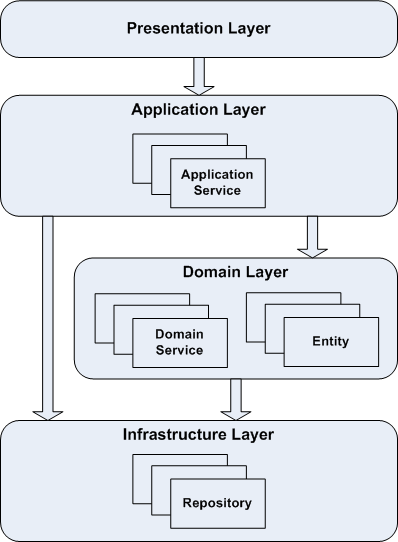
\includegraphics[height = 0.5\textwidth]{ddd-layer}
	\caption{Các tầng trong DDD}
\end{figure}

Domain-Driven Design chứa các khuôn mẫu (building blocks) có mục đích là để trình bày một số yếu tố chính của mô hình hóa hướng đối tượng và thiết kế phần mềm từ quan điểm của DDD.

Các khuôn mẫu cơ bản được sử dụng trong DDD gồm: Entities, Service, Value Object, Repository và Aggregate.

\subsubsection{Entities}

Trong các đối tượng của một phần mềm, có một nhóm các đối tượng có định danh riêng. Đối với những đối tượng này thì các thuộc tính của chúng có giá trị như thế nào không quan trọng bằng việc chúng tồn tại liên tục và xuyên suốt quá trình của hệ thống, thậm chí là sau cả khi đó. Chúng được gọi tên là thực thể - Entity.

Các Entities là sự kết hợp của dữ liệu và hành vi, như người dùng hoặc sản phẩm. Chúng có danh tính, nhưng đại diện cho các điểm dữ liệu với hành vi.

Lấy ví dụ, để tạo một lớp Person chứa thông tin về một người chúng ta có thể tạo Person với các trường như: tên, ngày sinh, nơi sinh v.v... Những thuộc tính này có thể coi là định danh của một người không? Tên thì không phải vì có thể có trường hợp trùng tên nhau, ngày sinh cũng không phải là định danh vì trong một ngày có rất nhiều người sinh ra, và nơi sinh cũng vậy. Một đối tượng cần phải được phân biệt với những đối tượng khác cho dù chúng có chung thuộc tính đi chăng nữa. Việc nhầm lẫn về định danh giữa các đối tượng có thể gây lỗi dữ liệu nghiêm trọng.

Đối với một người đó có thể là một tổ hợp của các thông tin như: tên, ngày sinh, nơi sinh, tên bố mẹ, địa chỉ hiện tại... Đối với một tài khoản ngân hàng thì số tài khoản là đủ để tạo định danh. Điểm mấu chốt ở đây là hệ thống có thể phân biệt hai đối tượng với hai định danh khác nhau một cách dễ dàng, hay hai đối tượng chung định danh có thể coi là một.

\begin{figure}[H]
	\centering
	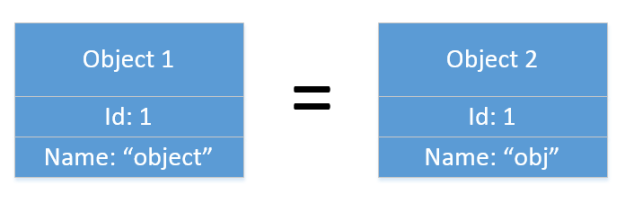
\includegraphics[width = 1\textwidth]{entity}
	\caption{Khuôn mẫu Entity}
\end{figure}

\subsubsection{Value objects}

Một đối tượng mà được dùng để mô tả các khía cạnh cố định của một domain, và không có định danh, được gọi tên là Value Object.

Value Object thể hiện những thành phần hoặc khái niệm của domain mà chỉ được biết bằng đặc điểm của nó. Chúng được dùng như mô tả của thành phần trong model, và không yêu cầu định danh. Value Object không cần định danh bởi vì chúng luôn kết hợp với một đối tượng khác và do đó luôn có thể hiểu được trong ngữ cảnh cụ thể.

Một điểm quan trọng là Value Object được xem như là bất biến, và không bao giờ được thay đổi trong vòng đời của mình. Ưu điểm của nó là nhờ không có định danh nên có thể tạo và xóa dễ dàng.

Value object có các thuộc tính, nhưng không thể tự tồn tại. Ví dụ: địa chỉ giao hàng có thể là một value object. Các hệ thống lớn và phức tạp có vô số entitiy và value object. Đó là lý do tại sao mô hình miền cần một số loại khuôn mẫu tiếp theo. Điều này sẽ đưa chúng vào các Aggregates hợp lý sẽ dễ quản lý hơn.

\subsubsection{Aggregates}

Những nhóm này được gọi là Aggregates. Chúng đại diện cho một tập hợp các đối tượng được kết nối với nhau, với mục tiêu coi chúng như các đơn vị. Hơn nữa, chúng cũng có một aggregate root. Đây là thực thể duy nhất mà bất kỳ đối tượng nào bên ngoài tổng thể đều có thể tham chiếu đến.

Entity và Value Object hình thành nên những mối quan hệ phức tạp trong domain model. Khi hệ thống lớn và có sự kết nối, tương tác giữa nhiều đối tượng, việc đảm bảo tính tương tranh và nhất quán trở nên khó khăn.

Do vậy, chúng ta cần sử dụng Aggregate. Một Aggregate là một nhóm các đối tượng, nhóm này có thể được xem như là một đơn vị thống nhất đối với các thay đổi dữ liệu. Một Aggregate được phân tách với phần còn lại của hệ thống, ngăn cách giữa các đối tượng nội tại và các đối tượng ở ngoài. Mỗi Aggregate có một "gốc" (Aggregate root), đó là một Entity và cũng là đối tượng duy nhất có thể truy cập từ phía ngoài của Aggregate. Gốc của Aggregate có thể chứa những tham chiếu đến các đối tượng khác trong Aggregate, và những đối tượng trong này có thể chứa tham chiếu đến nhau, nhưng các đối tượng ở ngoài chỉ có thể tham chiếu đến gốc của Aggreagte. Nếu như trong Aggregate có những Entity khác thì định danh của chúng là nội tại, chỉ mang ý nghĩa trong Aggregate.

\begin{figure}[H]
	\centering
	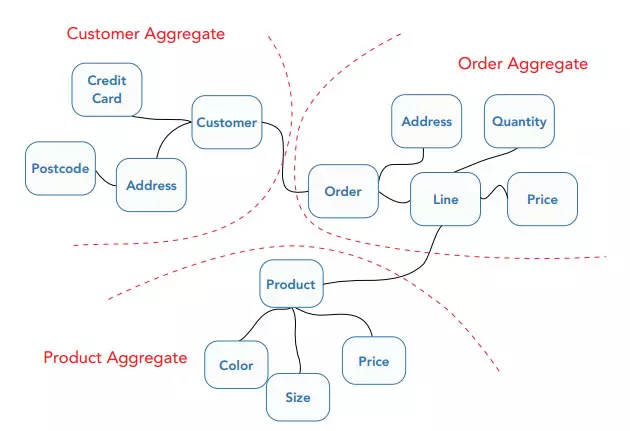
\includegraphics[width = 1\textwidth]{aggregate}
	\caption{Khuôn mẫu Aggregates}
\end{figure}

\subsubsection{Service}

Service là một lớp bổ sung cũng chứa logic nghiệp vụ. Nó là một phần của domain model, giống như các entity và value object. Đồng thời, dịch vụ ứng dụng là một lớp khác không chứa logic nghiệp vụ. Tuy nhiên, nó ở đây để điều phối hoạt động của ứng dụng, được đặt phía trên domain model.

Khi phân tích domain để xác định những đối tượng chính có trong mô hình, có thể bắt gặp những thành phần không dễ để có thể gán chúng cho một đối tượng nhất định nào đó. Tuy nhiên có một số hành vi trong domain lại không thuộc về một đối tượng nhất định nào cả. Chúng thể hiện cho những hành vi quan trọng trong domain nên không thể bỏ qua chúng hoặc gắn vào các Entity hay Value Object. Việc thêm hành vi này vào một đối tượng sẽ làm mất ý nghĩa của đối tượng đó, gán cho chúng những chức năng vốn không thuộc về chúng.

Đối với những hành vi như vậy trong domain, đó chính là một Service. Một Service không có trạng thái nội tại và nhiệm vụ của nó đơn giản là cung cấp các chức năng cho domain. Service có thể đóng một vai trò quan trọng trong domain, chúng có thể bao gồm các chức năng liên quan đến nhau để hỗ trợ cho các Entity và Value Object. Việc khai báo một Service một cách tường minh giúp phân biệt rõ các chức năng trong domain đó, giúp tách biệt rạch ròi khái niệm.

Một Service không nên bao gồm các thao tác vốn thuộc về các đối tượng của domain. Sẽ là không nên cứ có bất kỳ thao tác nào chúng ta cũng tạo một Service cho chúng. Chỉ khi một thao tác đóng một vai trò quan trọng trong domain ta mới cần tạo một Service để thực hiện.

\begin{figure}[H]
	\centering
	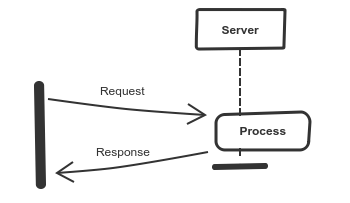
\includegraphics[width = 1\textwidth]{repository}
	\caption{Khuôn mẫu Service}
\end{figure}

\subsubsection{Repository}

Repository là một tập hợp các thực thể nghiệp vụ giúp đơn giản hóa cơ sở hạ tầng dữ liệu. Nó giải phóng domail model khỏi những lo ngại về cơ sở hạ tầng.

Mục đích của repository là để đóng gói tất cả các logic cần thiết để thu được các tham chiếu đối tượng. Các đối tượng domain sẽ không cần phải xử lý với cơ sở dữ liệu để lấy những tham chiếu cần thiết tới các đối tượng khác của domain. Chúng sẽ chỉ lấy nó từ Repository và model lấy lại được sự rõ ràng và tập trung.

Repository có thể lưu trữ các tham chiếu tới một vài đối tượng. Khi một đối tượng được khởi tạo, nó có thể được lưu lại trong Repository, và được lấy ra từ đây để có thể sử dụng sau này. Nếu phía client yêu cầu đối tượng từ Repository, và Repository không chứa chúng, nó có thể sẽ được lấy từ bộ nhớ. Dù bằng cách nào, các Repository hoạt động như một nơi lưu trữ các đối tượng cho việc truy xuất đối tượng toàn cục.

\begin{figure}[H]
	\centering
	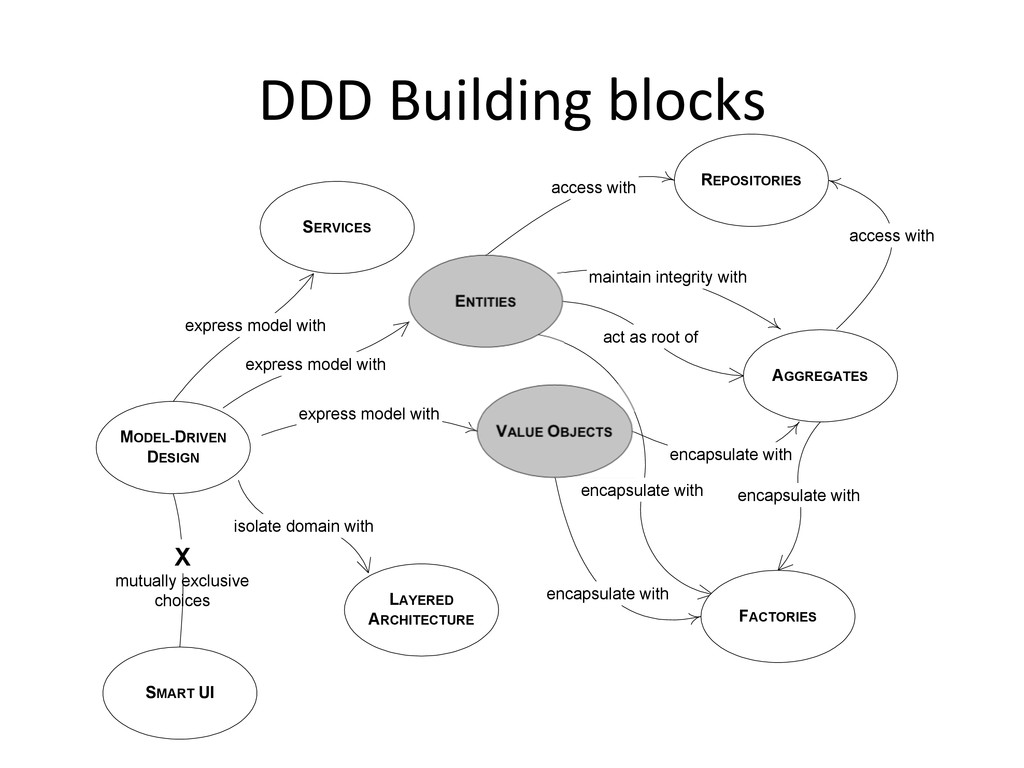
\includegraphics[width = 1\textwidth]{building-blocks}
	\caption{Các khuôn mẫu trong DDD}
\end{figure}

\subsection{Kiến trúc Onion}

Domain-driven design (DDD) là một cách tiếp cận để phát triển phần mềm cho các nhu cầu phức tạp bằng cách kết nối việc triển khai với một mô hình kinh doanh cốt lõi. DDD tập trung vào mô hình nghiệp vụ có hiểu biết phong phú về các quy trình và quy tắc của nghiệp vụ. Kiến trúc Onion thực hiện khái niệm này và tăng đáng kể chất lượng mã code, giảm độ phức tạp và cho phép các hệ thống doanh nghiệp phát triển.

Kiến trúc Onion được xây dựng trên mô hình nghiệp vụ trong đó các lớp được kết nối thông qua các interface. Ý tưởng là giữ các phụ thuộc bên ngoài càng xa càng tốt, nơi các thực thể nghiệp vụ và các quy tắc nghiệp vụ tạo thành phần cốt lõi của kiến trúc.

\begin{itemize}
	\item Nó cung cấp kiến trúc linh hoạt, bền vững và dễ mở rộng
	\item Các lớp được liên kết chặt chẽ và có sự phân tách rõ ràng
	\item Nó cung cấp khả năng bảo trì tốt hơn vì tất cả mã code phụ thuộc vào các lớp sâu hơn hoặc lớp trung tâm
	\item Cải thiện khả năng kiểm tra vì các kiểm tra có thể được tạo cho các lớp riêng biệt mà không ảnh hưởng đến các lớp khác
	\item Các công nghệ có thể dễ dàng thay đổi mà không ảnh hưởng đến nghiệp vụ lõi
\end{itemize}

Các tầng được biểu diễn thành dạng các vòng tròn đồng tâm. Đặc trưng của kiến trúc củ hành đó là một luật về sự ràng buộc giữa các tầng. Tầng bên ngoài chỉ phụ thuộc và gọi trực tiếp tầng bên trong. Các tầng thấp hơn không thể phụ thuộc vào các tầng bên ngoài.

\subsubsection{Nguyên lý}

Kiến trúc Onion bao gồm nhiều lớp đồng tâm giao thoa với nhau về phía lõi đại diện cho nghiệp vụ. Nó dựa trên sự đảo ngược của nguyên tắc điều khiển. Kiến trúc không tập trung vào công nghệ hay khuôn khổ mà là các mô hình nghiệp vụ thực tế. Nó dựa trên các nguyên tắc sau:

\begin{itemize}
	\bfitem{Sự phụ thuộc}{Các vòng tròn đại diện cho các lớp trách nhiệm khác nhau. Nói chung, càng đi sâu, các lớp càng tiến gần đến nghiệp vụ và các quy tắc kinh doanh. Các lớp bên ngoài đại diện cho các cơ chế và các lớp bên trong đại diện cho logic nghiệp vụ. Các lớp bên ngoài phụ thuộc vào các lớp bên trong và các lớp bên trong hoàn toàn không nhận biết được các lớp bên ngoài. Định dạng / cấu trúc dữ liệu có thể khác nhau giữa các lớp. Các định dạng dữ liệu lớp bên ngoài không được sử dụng bởi các lớp bên trong}
	\bfitem{Bao bọc dữ liệu}{Mỗi lớp bao bọc hoặc ẩn các chi tiết triển khai bên trong và cung cấp API cho lớp bên ngoài. Tất cả các lớp cũng cần cung cấp thông tin để cho các lớp bên trong sử dụng một cách thuận tiện. Mục đích là giảm thiểu sự kết hợp giữa các lớp và tối đa hóa sự kết hợp trong một lát dọc giữa các lớp. Điều này đảm bảo sự tập trung vào mô hình nghiệp vụ mà không cần lo lắng quá nhiều về chi tiết triển khai}
	\bfitem{Tách mối quan tâm}{Ứng dụng được chia thành các lớp trong đó mỗi lớp có một tập hợp các trách nhiệm và giải quyết các mối quan tâm riêng biệt. Mỗi lớp hoạt động như các modules/package/namespace tên trong ứng dụng}
	\bfitem{Rằng buộc}{Rằng buộc thấp trong đó một module tương tác với một module khác và không cần quan tâm đến các phần bên trong của module đó. Tất cả các lớp bên trong không cần quan tâm đến việc triển khai của các lớp bên ngoài}
\end{itemize}

\subsubsection{Các lớp của Kiến trúc Onion}

\begin{itemize}
	\bfitem{Lớp nghiệp vụ}{Ở phần trung tâm của Kiến trúc Onion, lớp miền tồn tại; lớp này đại diện cho các đối tượng nghiệp vụ và hành vi. Ý tưởng là có tất cả các đối tượng miền của bạn ở cốt lõi này. Nó chứa tất cả các đối tượng miền ứng dụng. Bên cạnh các đối tượng miền, bạn cũng có thể có các giao diện miền. Các thực thể miền này không có bất kỳ phụ thuộc nào}
	\bfitem{Lớp kho lưu trữ}{Lớp này tạo ra một sự trừu tượng giữa các thực thể miền và logic nghiệp vụ của một ứng dụng. Trong lớp này, thường thêm các giao diện cung cấp hành vi lưu và truy xuất đối tượng thường bằng cách liên quan đến cơ sở dữ liệu. Lớp này bao gồm mẫu truy cập dữ liệu, là một cách tiếp cận kết hợp lỏng hơn để truy cập dữ liệu. Chúng tôi cũng tạo một kho lưu trữ chung và thêm các truy vấn để truy xuất dữ liệu từ nguồn, ánh xạ dữ liệu từ nguồn dữ liệu sang một thực thể kinh doanh và duy trì những thay đổi trong thực thể kinh doanh đối với nguồn dữ liệu}
	\bfitem{Lớp dịch vụ}{Lớp Dịch vụ giữ các giao diện với các hoạt động phổ biến, chẳng hạn như Thêm, Lưu, Chỉnh sửa và Xóa. Ngoài ra, lớp này được sử dụng để giao tiếp giữa lớp UI và lớp kho lưu trữ. Lớp Dịch vụ cũng có thể giữ logic nghiệp vụ cho một thực thể. Trong lớp này, các giao diện dịch vụ được giữ với quá trình triển khai của nó, giữ cho sự liên kết lỏng và tách biệt các mối quan tâm trong tâm trí}
	\bfitem{Lớp giao diện người dùng}{Đây là lớp ngoài cùng và giữ các mối quan tâm ngoại vi như giao diện người dùng và các thử nghiệm. Đối với một ứng dụng Web, nó đại diện cho dự án Web API hoặc Unit Test. Lớp này có sự triển khai của nguyên tắc tiêm phụ thuộc để ứng dụng xây dựng một cấu trúc liên kết lỏng và có thể giao tiếp với lớp bên trong thông qua các giao diện}
\end{itemize}

\begin{figure}[H]
	\centering
	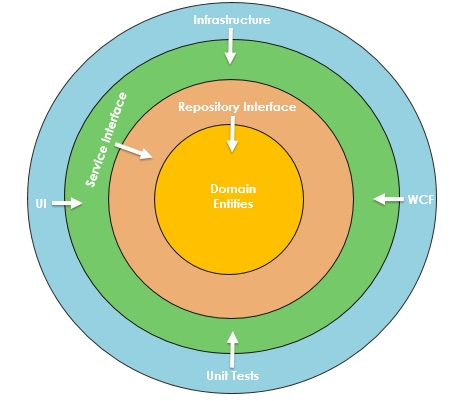
\includegraphics[width = 0.7\textwidth]{onion_architecture}
	\caption{Các lớp của Kiến trúc Onion}
\end{figure}

\section{Kiến trúc tổng quan hệ thống}

\subsection{Hệ thống frontend}

\subsubsection{Hệ thống Trang}

Hệ thống frontend có các hệ thống Trang sau đây: Product, Layer, Experiment và Test Group. Mỗi hệ thống Trang bao gồm có hệ thống Đường dẫn, mỗi Đường dẫn có một nhiệm vụ cụ thể được ghi chú trong Chú thích.

Mỗi thực thể đều có một hệ thống Trang nhằm mục đích cho người dùng có thể khởi tạo, cập nhập và thay đổi theo ý muốn. Ngoài ra người dùng có thể có cái nhìn toàn cảnh với mỗi thực thể.

\begin{table}[H]
	\centering
	\begin{tabular}{|c|l|p{5cm}|}
		\hline
		Trang                    & Đường dẫn                                       & Chú thích                \\ \hline
		\multirow{4}{*}{Product} & /product                                        & Hiển thị toàn bộ Product \\ \cline{2-3}
		                         & /product/new                                    & Khởi tạo Product         \\ \cline{2-3}
		                         & /product/:id                                    & Hiển thị Product         \\ \cline{2-3}
		                         & /product/:id/update                             & Cập nhật Product         \\ \hline
		\multirow{4}{*}{Layer}
		                         & /product/:id/layer/new                          & Khởi tạo Layer           \\ \cline{2-3}
		                         & /product/:id/layer/:id                          & Hiển thị Layer           \\ \cline{2-3}
		                         & /product/:id/layer/:id/update                   & Cập nhật Layer           \\ \hline
		\multirow{4}{*}{Experiment}
		                         & /product/:id/layer/:id/exp/new                  & Khởi tạo Experiment      \\ \cline{2-3}
		                         & /product/:id/layer/:id/exp/:id                  & Hiển thị Layer           \\ \cline{2-3}
		                         & /product/:id/layer/:id/exp/:id/update           & Cập nhật Layer           \\ \hline
		\multirow{4}{*}{Group}
		                         & /product/:id/layer/:id/exp/:id/group/new        & Khởi tạo Test Group      \\ \cline{2-3}
		                         & /product/:id/layer/:id/exp/:id/group/:id        & Hiển thị Test Group      \\ \cline{2-3}
		                         & /product/:id/layer/:id/exp/:id/group/:id/update & Cập nhật Test Group      \\ \hline
	\end{tabular}
	\caption{Hệ thống Trang}
\end{table}

Với mỗi Trang, các thông tin sẽ được hiển thị như sau:

\begin{itemize}
	\bfitem{/product}{}
	\begin{itemize}
		\item Toàn bộ Product
		\item Id của mỗi Product
		\item Tên của mỗi Product
		\item Số lượng Layer trong mỗi Product
	\end{itemize}
	\bfitem{/product/:id}{}
	\begin{itemize}
		\item Tên của Product
		\item Số lượng Layer của Product
		\item Số lượng Experiment của Product
		\item Toàn bộ Layer của Product
		      \begin{itemize}
			      \item Id của mỗi Layer
			      \item Tên của mỗi Layer
			      \item Hash stragety của mỗi Layer
			      \item Số lượng Experiment của mỗi Layer
		      \end{itemize}
	\end{itemize}
	\bfitem{/product/:id/layer/:id}{}
	\begin{itemize}
		\item Tên của Layer
		\item Hash stragety của Layer
		\item Traffic còn lại của Layer
		\item Số lượng Experiment của Layer
		\item Toàn bộ Experiment của Layer
		      \begin{itemize}
			      \item Id của mỗi Experiment
			      \item Tên của mỗi Experiment
			      \item Traffic của mỗi Experiment
			      \item Trạng thái của mỗi Experiment
			      \item Thời điểm bắt đầu của mỗi Experiment
			      \item Thời điểm kết thúc của mỗi Experiment
			      \item Số lượng Test Group của mỗi Experiment
		      \end{itemize}
	\end{itemize}
	\bfitem{/product/:id/layer/:id/exp/:id}{}
	\begin{itemize}
		\item Tên của Experiment
		\item Traffic của Experiment
		\item Trạng thái của Experiment
		\item Thời điểm bắt đầu của Experiment
		\item Thời điểm kết thúc của Experiment
		\item Số lượng Test Group của Experiment
		\item Toàn bộ Test Group của Experiment
		      \begin{itemize}
			      \item Id của mỗi Test Group
			      \item Tên của mỗi Test Group
			      \item Toàn bộ Parameter của Test Group
			            \begin{itemize}
				            \item Tên của mỗi Parameter
				            \item Giá trị của mỗi Parameter
			            \end{itemize}
		      \end{itemize}
	\end{itemize}
\end{itemize}

\subsubsection{Các thành phần}

Hệ thống frontend gồm các thành phần sau: Types, Pages, Services và Components

\begin{itemize}
	\bfitem{Types}{Mục đích là tổng hợp các thực thể ở tầng Frontend, bao gồm hai loại là Thực thể gốc và nội dung khi nhận/gửi API}
	\bfitem{Pages}{Là thành phần xử lý hệ thống Trang, mỗi file sẽ là một hệ thống Trang khác nhau}
	\bfitem{Services}{Là thành phần xử lý hệ thống thông tin cho toàn bộ hệ thống Frontend, bao gồm cả việc nhận, gửi dữ liệu từ Server}
	\bfitem{Components}{Chứa các thành phần chung giữa các trang}
\end{itemize}

% \begin{figure}[H]
% 	\centering
% 	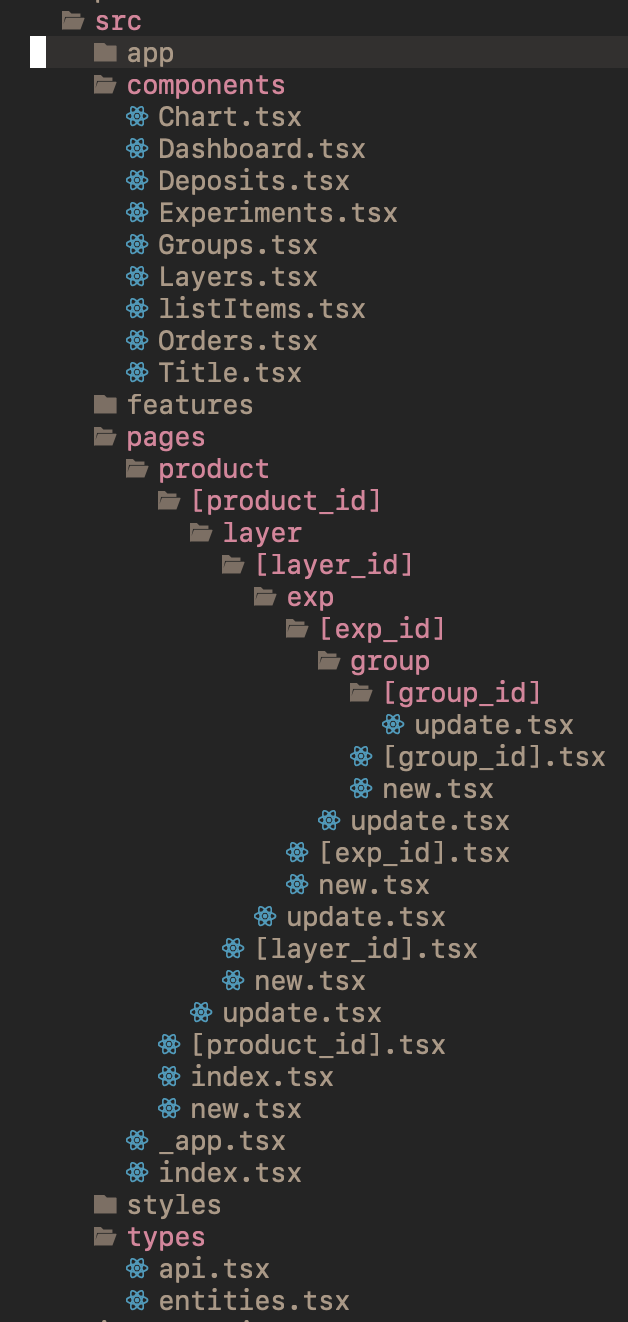
\includegraphics[width = 0.7\textwidth]{frontend-structure}
% 	\caption{Hệ thống Frontend}
% \end{figure}

\subsection{Hệ thống backend}

\subsubsection{Các thành phần}

Các thành phần trong hệ thống backend đảm nhiệm một nhiệm vụ riêng biệt gồm các thành phần sau:

\begin{itemize}
	\bfitem{Service}{Là thành phần xử lý hệ thống HTTP, chuyên nhận và phản hồi các truy cập từ hệ thống Frontend}
	\begin{itemize}
		\bfitem{Summary}{Gửi trả toàn bộ dữ liệu của các A/B Test}
		\bfitem{Abtest}{Thực hiện và gửi trả A/B Test}
		\bfitem{Entity}{Thực hiện khởi tạo hoặc cập nhật các thực thể, gửi trả kết quả}
	\end{itemize}
	\bfitem{Storage}{Là thành phần tổng hợp thông tin cho tầng Service}
	\begin{itemize}
		\bfitem{Summary}{Tổng hợp toàn bộ dữ liệu của các A/B Test}
		\bfitem{Entity}{Khởi tạo hoặc cập nhật các thực thể}
	\end{itemize}
	\bfitem{Database}{Là thành phần quản lý dữ liệu cho tầng Storage}
	\begin{itemize}
		\bfitem{Entity}{Khởi tạo hoặc cập nhật các thực thể}
	\end{itemize}
	\bfitem{Types}{Tổng hợp các thực thể ở tầng Backend, bao gồm 2 loại là: thực thể gốc và nội dung khi nhận/gửi API}
	\begin{itemize}
		\bfitem{Entity}{Dữ liệu của các thực thể}
		\bfitem{API}{Dữ liệu nội dung cho các yêu cầu/kết quả khi truy cập}
	\end{itemize}
	\bfitem{Abtest}{Thực hiện A/B Test}
\end{itemize}

\begin{figure}[H]
	\centering
	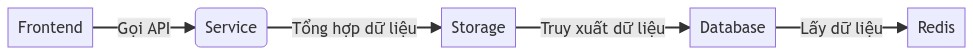
\includegraphics[width = 1\textwidth]{backend}
	\caption{Hệ thống Backend}
\end{figure}

\subsubsection{Hệ thống API}

Mỗi thực thể có chức năng riêng biệt nhau. Hệ thống đường dẫn bao gồm các thực thể sau:

\begin{table}[H]
	\centering
	\begin{tabular}{|l|l|l|}
		\hline
		\textbf{Thực thể}           & \textbf{Đường dẫn} & \textbf{Chú thích}                          \\ \hline
		Summary                     & /summary           & Gọi toàn bộ thông tin của hệ thống A/B Test \\ \hline
		AbTest                      & /abtest            & Thực hiện A/B Test                          \\ \hline
		\multirow{2}{*}{Product}    & /product/create    & Khởi tạo Product mới                        \\ \cline{2-3}
		                            & /product/update    & Cập nhật Product                            \\ \hline
		\multirow{2}{*}{Layer}      & /layer/create      & Khởi tạo Layer mới                          \\ \cline{2-3}
		                            & /layer/update      & Cập nhật Layer                              \\ \hline
		\multirow{2}{*}{Experiment} & /exp/create        & Khởi tạo Experiment mới                     \\ \cline{2-3}
		                            & /exp/update        & Cập nhật Experiment                         \\ \hline
		\multirow{2}{*}{Test Group} & /group/create      & Khởi tạo Test Group mới                     \\ \cline{2-3}
		                            & /group/update      & Cập nhật Test Group mới                     \\ \hline
	\end{tabular}
	\caption{Hệ thống đường dẫn}
\end{table}

Với mỗi API, sẽ có cấu trúc về yêu cầu và kết quả như sau:

\begin{itemize}
	\bfitem{Summary}{}
	\begin{itemize}
		\bfitem{Kết quả}{Toàn bộ Product, trong Product có toàn bộ Layer của Product đó, v.v}
	\end{itemize}
	\bfitem{AbTest}{}
	\begin{itemize}
		\bfitem{Yêu cầu}{Thông tin của user và product nào cần thực hiện A/B Test}
		\begin{itemize}
			\bfitem{product id}{Id của Product cần thực hiện A/B Test}
			\bfitem{user id}{Id của người dùng}
			\bfitem{session id}{Id của sesion mà người dùng đang sử dụng}
		\end{itemize}
		\bfitem{Kết quả}{Thông tin của các A/B Test thử nghiệm với user}
		\begin{itemize}
			\bfitem{product id}{Id của Product đang thực hiện A/B Test}
			\bfitem{layer id}{Id của Layer sẽ thực hiện A/B Test này}
			\bfitem{experiment id}{Id của Experiment sẽ thực hiện A/B Test này}
			\bfitem{test group id}{Id của Test Group sẽ thực hiện A/B Test này}
			\bfitem{parameters}{Tên và giá trị của các Parameter}
		\end{itemize}
	\end{itemize}
	\bfitem{Product}{}
	\begin{itemize}
		\bfitem{Create}{Khởi tạo một Product}
		\begin{itemize}
			\bfitem{Yêu cầu}{Nội dung của Product đó}
			\bfitem{Kết quả}{Nội dung của Product đó cộng thêm mã id định danh}
		\end{itemize}
		\bfitem{Update}{Cập nhật một Product}
		\begin{itemize}
			\bfitem{Yêu cầu}{Nội dung của Product đó}
			\bfitem{Kết quả}{Nội dung của Product đó}
		\end{itemize}
	\end{itemize}
	\bfitem{Layer}{}
	\begin{itemize}
		\bfitem{Create}{Khởi tạo một Layer}
		\begin{itemize}
			\bfitem{Yêu cầu}{Nội dung của Layer đó}
			\bfitem{Kết quả}{Nội dung của Layer đó cộng thêm mã id định danh}
		\end{itemize}
		\bfitem{Update}{Cập nhật một Layer}
		\begin{itemize}
			\bfitem{Yêu cầu}{Nội dung của Layer đó}
			\bfitem{Kết quả}{Nội dung của Layer đó}
		\end{itemize}
	\end{itemize}
	\bfitem{Experiment}{}
	\begin{itemize}
		\bfitem{Create}{Khởi tạo một Experiment}
		\begin{itemize}
			\bfitem{Yêu cầu}{Nội dung của Experiment đó}
			\bfitem{Kết quả}{Nội dung của Experiment đó cộng thêm mã id định danh}
		\end{itemize}
		\bfitem{Update}{Cập nhật một Experiment}
		\begin{itemize}
			\bfitem{Yêu cầu}{Nội dung của Experiment đó}
			\bfitem{Kết quả}{Nội dung của Experiment đó}
		\end{itemize}
	\end{itemize}
	\bfitem{Test Group}{}
	\begin{itemize}
		\bfitem{Create}{Khởi tạo một Test Group}
		\begin{itemize}
			\bfitem{Yêu cầu}{Nội dung của Test Group đó}
			\bfitem{Kết quả}{Nội dung của Test Group đó cộng thêm mã id định danh}
		\end{itemize}
		\bfitem{Update}{Cập nhật một Test Group}
		\begin{itemize}
			\bfitem{Yêu cầu}{Nội dung của Test Group đó}
			\bfitem{Kết quả}{Nội dung của Test Group đó}
		\end{itemize}
	\end{itemize}
\end{itemize}

\subsection{Biểu đồ tuần tự}

\subsubsection{Biểu đồ tuần tự chung}

Biểu đồ tuần tự chung biểu thị việc khởi tạo và sử dụng A/B Test.

\begin{figure}[H]
	\centering
	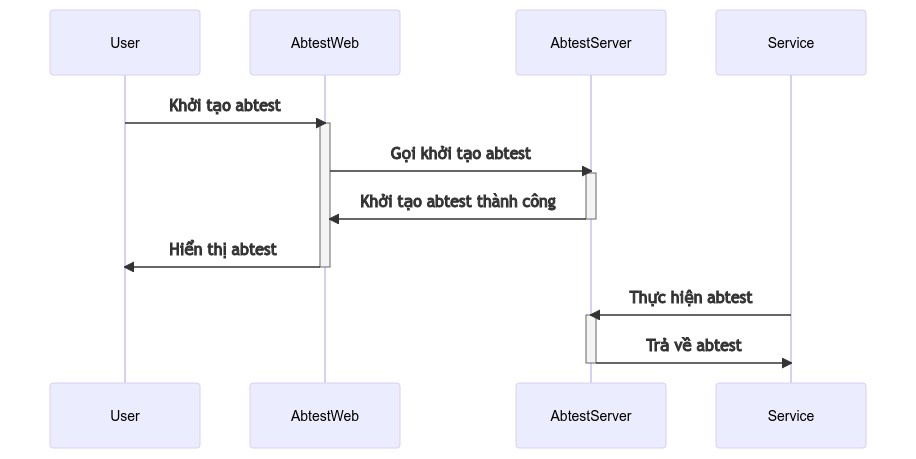
\includegraphics[width = 1\textwidth]{overview-sequence}
	\caption{Biểu đồ tuần tự chung}
\end{figure}

\subsubsection{Biểu đồ tuần tự khởi tạo A/B Test}

Biểu đồ tuần tự khởi tạo A/B Test

\begin{figure}[H]
	\centering
	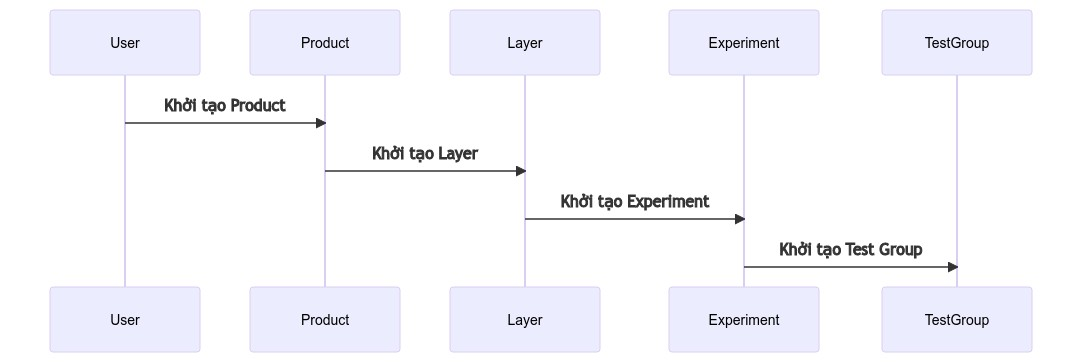
\includegraphics[width = 1\textwidth]{abtest-sequence}
	\caption{Biểu đồ tuần tự khởi tạo A/B Test}
\end{figure}

\section{Mô hình cơ sở dữ liệu}

Mô hình cơ sở dữ liệu của hệ thống mô tả cụ thể các đặc tính của mỗi thực thể, ngoài ra mô tả
cách lưu trữ các thực thể và các mối quan hệ tương quan trong cơ sở dữ liệu.

\subsection{Các thực thể}

Các thực thể bao gồm: Product, Layer, Experiment và Test Group.

\subsubsection{Product}

Product là thực thể lớn nhất, chỉ có chức năng phân tách theo nhu cầu sử dụng nên chỉ có 2 trường như sau:
\begin{table}[H]
	\centering
	\begin{tabular}{|l|l|l|}
		\hline
		Trường & Loại   & Chú thích       \\ \hline
		id     & int    & Mã id định danh \\ \hline
		name   & string & Tên của Product \\ \hline
	\end{tabular}
	\caption{Thuộc tính của Product}
\end{table}

Cấu hình khi được lưu xuống cơ sở dữ liệu:

\begin{itemize}
	\bfitem{Key}{product::[id]}
	\bfitem{Value}{binary (nén bởi JSON)}
	\bfitem{Command}{SET, GET}
\end{itemize}

\subsubsection{Layer}

\begin{table}[H]
	\centering
	\begin{tabular}{|l|l|l|}
		\hline
		Trường & Loại   & Chú thích       \\ \hline
		id     & int    & Mã id định danh \\ \hline
		name   & string & Tên của Layer   \\ \hline
		type   & int    & Loại của Layer  \\ \hline
	\end{tabular}
	\caption{Thuộc tính của Layer}
\end{table}

Cấu hình khi được lưu xuống cơ sở dữ liệu:

\begin{itemize}
	\bfitem{Key}{layer::[id]}
	\bfitem{Value}{binary (nén bởi JSON)}
	\bfitem{Command}{SET, GET}
\end{itemize}

\subsubsection{Experiment}

\begin{table}[H]
	\centering
	\begin{tabular}{|l|l|l|}
		\hline
		Trường      & Loại   & Chú thích          \\ \hline
		id          & int    & Mã id định danh    \\ \hline
		name        & string & Tên của Experiment \\ \hline
		traffic     & int    & Số lượng traffic   \\ \hline
		start\_time & int    & Thời điểm bắt đầu  \\ \hline
		end\_time   & int    & Thời điểm kết thúc \\ \hline
		status      & int    & Trạng thái         \\ \hline
	\end{tabular}
	\caption{Thuộc tính của Experiment}
\end{table}

Cấu hình khi được lưu xuống cơ sở dữ liệu:

\begin{itemize}
	\bfitem{Key}{exp::[id]}
	\bfitem{Value}{binary (nén bởi JSON)}
	\bfitem{Command}{SET, GET}
\end{itemize}

\subsubsection{Test Group}

\begin{table}[H]
	\centering
	\begin{tabular}{|l|l|l|}
		\hline
		Trường    & Loại   & Chú thích                \\ \hline
		id        & int    & Mã id định danh          \\ \hline
		parameter & string & Parameter của Test Group \\ \hline
		value     & string & Value của Parameter      \\ \hline
	\end{tabular}
	\caption{Thuộc tính của Test Group}
\end{table}

Cấu hình khi được lưu xuống cơ sở dữ liệu:

\begin{itemize}
	\bfitem{Key}{group::[id]}
	\bfitem{Value}{binary (nén bởi JSON)}
	\bfitem{Command}{SET, GET}
\end{itemize}

\subsection{Mối quan hệ giữa các thực thể}

Giữa các thực thể có các mối quan hệ lẫn nhau, vì vậy ngoài việc lưu trữ các thực thể dưới
cơ sở dữ liệu, cũng cần lưu trữ mối quan hệ giữa chúng.

\subsubsection{Tổng hợp các Product}

Khi cần query tất cả các Product hiện có, chỉ cần lưu các id của product vào một chỗ.

Cấu hình khi được lưu xuống cơ sở dữ liệu:

\begin{itemize}
	\bfitem{Key}{product::ids}
	\bfitem{Value}{các id của product}
	\bfitem{Command}{SADD, SMEMBERS}
\end{itemize}

\subsubsection{Giữa Product và Layer}

Mỗi Product có nhiều Layer, khi cần query tất cả các Layer dưới một Product, chỉ cần lưu
các id của layer vào một chỗ.

Cấu hình khi được lưu xuống cơ sở dữ liệu:

\begin{itemize}
	\bfitem{Key}{product::[id]::layers}
	\bfitem{Value}{các id của Layer}
	\bfitem{Command}{SADD, SMEMBERS}
\end{itemize}

\subsubsection{Giữa Layer và Experiment}

Mỗi Layer có nhiều Experiment, khi cần query tất cả các Experiment dưới một Layer, chỉ cần lưu
các id của Experiment vào một chỗ.

Cấu hình khi được lưu xuống cơ sở dữ liệu:

\begin{itemize}
	\bfitem{Key}{layer::[id]::exps}
	\bfitem{Value}{các id của Experiment}
	\bfitem{Command}{SADD, SMEMBERS}
\end{itemize}

\subsubsection{Giữa Experiment và Test Group}

Mỗi Experiment có nhiều Test Group, khi cần query tất cả các Test Group dưới một Experiment, chỉ cần lưu
các id của Test Group vào một chỗ.

Cấu hình khi được lưu xuống cơ sở dữ liệu:

\begin{itemize}
	\bfitem{Key}{exp::[id]::groups}
	\bfitem{Value}{các id của Test Group}
	\bfitem{Command}{SADD, SMEMBERS}
\end{itemize}

\subsection{Id Generator}

Mỗi thực thể đều yêu cầu một mã ID định danh, do đó cơ sở dữ liệu cũng cần được sử dụng để mỗi
khi tạo một thực thể mới có thể có một mã ID định danh mới.

Cấu hình khi được lưu xuống cơ sở dữ liệu:

\begin{itemize}
	\bfitem{Key}{product::id, layer::id, exp::id, group::id}
	\bfitem{Value}{Mã ID đang sử dụng hiện tại}
	\bfitem{Command}{INCR}
\end{itemize}


\chapter{TRIỂN KHAI VÀ THỰC NGHIỆM}
\chapter{TRIỂN KHAI VÀ THỰC NGHIỆM}

\section{Ứng dụng Domain Driven Design}

\subsection{Phân tầng}

\subsection{Định nghĩa lớp}

% \subsubsection{Tầng Application}
%
% \subsubsection{Tầng Domain}
%
% \subsubsection{Tầng Infrastructure}

\section{Triển khai chi tiết Use case}

\subsection{Use case khởi tạo A/B Test}

\subsubsection{Bước 1: Xác định ngữ cảnh}

\begin{itemize}
	\item Phía frontend gồm có: page để hiển thị và khởi tạo các thực thể
	\item Phía backend gồm có: Service, Storage, Database
\end{itemize}

\subsubsection{Bước 2: Xác định các trường dữ liệu}

\begin{itemize}
	\item Product: tên product
	\item Layer: tên layer, loại của layer
	\item Experiment: tên experiment, số lượng traffic, ngày bắt đầu và ngày kết thúc
	\item Test Group: tên của parameter, giá trị của parameter
\end{itemize}

\subsubsection{Bước 3: Xử lý nghiệp vụ}

\begin{itemize}
	\item Nhập dữ liệu trên website
	\item Frontend gọi API của Service
	\item Service gọi hàm tạo thực thể của Storage
	\item Storage gọi hàm tạo thực thể của Database
	\item Database thực hiện khởi tạo dữ liệu trên Cơ sở dữ liệu
	\item Cơ sở dữ liệu thực hiện thành công và gửi trả dữ liệu cho Database
	\item Database gửi trả dữ liệu cho Storage
	\item Storage gửi trả dữ liệu cho Service
	\item Service gửi trả dữ liệu cho Frontend
	\item Frontend thông báo thành công cho người dùng
\end{itemize}

\subsection{Use case sử dụng A/B Test}

\subsubsection{Bước 1: Xác định ngữ cảnh}

\begin{itemize}
	\item Phía frontend gồm có: page để hiển thị và khởi tạo các thực thể
	\item Phía backend gồm có: Service, Storage, Database
\end{itemize}

\subsubsection{Bước 2: Xác định các trường dữ liệu}

\begin{itemize}
	\item Product: Id của product
	\item UserID: Id của người dùng
	\item SessionID: session của request
\end{itemize}

\subsubsection{Bước 3: Xử lý nghiệp vụ}

\begin{itemize}
	\item Từ phía người dùng, thực hiện một request bất kỳ đến abtest API của Service
	\item Service gọi hàm tạo thực hiện abtest của Storage
	\item Storage gọi truy xuất thông tin của Product từ Database
	\item Database thực hiện truy xuất những dữ liệu cần trên Cơ sở dữ liệu
	\item Cơ sở dữ liệu thực hiện thành công và gửi trả dữ liệu cho Database
	\item Database gửi trả dữ liệu cho Storage
	\item Storage thực hiện abtest dựa trên những dữ liệu đang có và trả về cho Service
	\item Service gửi trả dữ liệu cho người dùng
\end{itemize}

\section{Triển khai kiểm thử thích hợp}

Việc kiểm thử phần mềm là quan trọng vì những lý do sau:

\begin{itemize}
	\item Kiểm thử chỉ ra sai sót của sản phẩm trong giai đoạn phát triển, đồng thời đảm bảo chất lượng sản phẩm trong tương lai.
	\item Kiểm thử đảm bảo kết quả cuối cùng đáp ứng các yêu cầu kinh doanh và người sử dụng.
\end{itemize}

Unit testing và integration testing:

\begin{table}[H]
	\centering
	\begin{tabular}{|p{8cm}|p{8cm}|}
		\hline
		\textbf{Unit testing}                                                                                                                                     & \textbf{Integration testing}                                                                                                                 \\ \hline
		Kiểm thử đơn vị là để kiểm tra từng phần của module riêng lẻ và quan sát rằng các bộ phận riêng lẻ đang hoạt động như mong đợi.                           & Kiểm thử tích hợp là tích hợp tất cả các module vào ứng dụng và kiểm tra chúng như một nhóm để xem chúng có hoạt động như mong đợi hay không \\ \hline
		Kiểm thử đơn vị còn được gọi là kiểm thử hộp trắng vì nó đòi hỏi kiến thức về mã code và luồng điều khiển trong chương trình.                             & Kiểm thử tích hợp còn được gọi là kiểm thử hộp đen, chúng ta không động đến mã code mà chỉ tập trung vào đầu vào đã cho và đầu ra mong đợi.  \\ \hline
		Unit testing có thể được thực hiện bất cứ lúc nào nhưng luôn luôn thực hiện trước khi kiểm thử tích hợp.                                                  & Integration Testing được thực hiện sau khi kiểm thử đơn vị nhưng trước khi kiểm thử hệ thống.                                                \\ \hline
		Unit Testing chỉ kiểm tra chức năng của các module ở cấp độ đơn vị và không thể bắt được các lỗi mức tích hợp hoặc bất kỳ vấn đề nào trong toàn hệ thống. & Các lỗi trong kiểm thử tích hợp được phát hiện sau khi các module được tích hợp để xây dựng hệ thống tổng thể.                               \\ \hline
		Chủ yếu tập trung vào chức năng của một module riêng lẻ.                                                                                                  & Chủ yếu tập trung vào tích hợp các module.                                                                                                   \\ \hline
		Unit Testing thường được thực hiện bởi các developers.                                                                                                    & Integration Testing được thực hiện bởi người kiểm thử(Tester).                                                                               \\ \hline
		Lỗi phát hiện thường đơn giản khi thử nghiệm đơn vị.                                                                                                      & Lỗi phát hiện thường khó khăn khi thử nghiệm tích hợp.                                                                                       \\ \hline
		Chi phí bảo trì kiểm thử đơn vị là rất ít vì nó được duy trì và mức đơn vị.                                                                               & Kiểm thử tích hợp bảo trì là khá tốn kém vì nó đòi hỏi phải thiết lập môi trường riêng biệt.                                                 \\ \hline
		Kiểm thử đơn vị không xác minh xem mã code có hoạt động như mong đợi với các phụ thuộc bên ngoài hay không.                                               & Kiểm thử tích hợp giúp xác minh rằng mã code hoạt động như mong đợi với các phụ thuộc bên ngoài.                                             \\ \hline
	\end{tabular}
\end{table}

Quy trình kiểm thử gồm 5 bước triển khai: Khởi tạo môi trường, chuẩn bị dữ liệu người dùng, gọi API, kiểm tra dữ liệu trả về, xóa môi trường.

% \subsection{Mô tả Integration test với một service cụ thể}

Sau đây sẽ thực hiện thử nghiệm với việc khởi tạo một A/B Test.

\begin{itemize}
	\item Chuẩn bị môi trường
	\item Xác định danh sách các API cần test
	      \begin{itemize}
		      \item Khởi tạo Product mới
		      \item Khởi tạo Layer mới
		      \item Khởi tạo Experiment mới
		      \item Khởi tạo Test Group mới
	      \end{itemize}
	\item Chuẩn bị các testcase bao gồm:
	      \begin{itemize}
		      \item API cần test
		      \item Dữ liệu đầu vào
		      \item Dữ liệu đầu ra mong muốn
		      \item Kết quả test
	      \end{itemize}
\end{itemize}

Viết code cho từng ca kiểm thử theo tập ca kiểm thử được chuẩn bị. Bảng ca kiểm thử được trình bày file ngoài.

Xóa trắng cơ sở dữ liệu sau mỗi vòng test.

% \section{Thực nghiệm}


\chapter{KẾT LUẬN VÀ HƯỚNG PHÁT TRIỂN}
\chapter{KẾT LUẬN VÀ HƯỚNG PHÁT TRIỂN}

Trong chương cuối cùng, chúng tôi ngắn ngọn kết luận kết quả đạt được của khóa luận, những hạn chế khi thực hiện đề tài và những hướng phát triển sắp tới.

\section{Kết quả đạt được}

Đề tài dự án đã tiến hành nghiên cứu về quy trình nghiệp vụ, các công nghệ và công cụ, đặc biệt là Domain Driven Design vào xây dựng hệ thống Abtest trong Quảng Cáo.

Việc thực hiện đề tài dự án giúp hiểu sâu hơn về nghiệp vụ quảng cáo, cách thức phân tích hệ thống và triển khai thực hiện các công nghệ cùng nhau.

\section{Hạn chế khi thực hiện đề tài}

Thứ nhất là do thiếu kiến thức quảng cáo nên khi triển khai nghiệp vụ còn nhiều sai sót và sửa đổi nhiều lần.

Thứ hai là do thời gian có hạn nên các module được cài đặt mới chỉ ở mức sơ khai. Còn tồn tại các hạn chế như chưa thực hiện việc quản lý kết quả abtest để thể hiện đúng chức năng nhất của một hệ thống abtest.

\section{Hướng phát triển}

Phát triển chức năng quản lý kết quả abtest để thành một sản phẩm trong hệ thống quảng cáo hoàn chỉnh.

Áp dụng các module đã xây dựng cho các hệ thống khác ngoài hệ thống abtest.


\end{document}
